\documentclass[11pt,a4paper,spanish]{book}
\usepackage{estilo_unir-1}
\usepackage{apacite}

\usepackage{hyperref}
\numberwithin{equation}{chapter}
%\usepackage{caption}
\numberwithin{figure}{chapter}
%\usepackage{chngcntr}
%\counterwithin{equation}{chapter}
%\counterwithin{figure}{chapter}
%\counterwithin{table}{chapter}
%\renewcommand\theequation{\thechapter.\arabic{equation}}
%\renewcommand\thefigure{\thechapter.\arabic{figure}}
%\renewcommand\thetable{\thechapter.\arabic{table}}
%\renewcommand\theequation{\thechapter.\arabic{equation}}
%\counterwithin{figure}{chapter}
%\counterwithin{table}{chapter}
%\renewcommand\thefigure{\thechapter.\arabic{figure}}
%\renewcommand\thetable{\thechapter.\arabic{table}}
%\renewcommand\thefigure{\thechapter.\arabic{figure}}
%\makeatletter
%\renewcommand\p@figure{\thechapter..\arabic{figure}}
%\makeatother


% para tablas
\usepackage{tabularx}
\usepackage{float} % en el preámbulo
\usepackage[font=small,labelfont=bf,labelsep=newline]{caption}
\captionsetup{justification=raggedright, singlelinecheck=false}



\usepackage{xcolor}
\usepackage{listings}
\lstset{
      language=Python,
      basicstyle=\ttfamily\footnotesize,
      keywordstyle=\color{blue},
      commentstyle=\color{gray},
      stringstyle=\color{red},
      numbers=left,
      numberstyle=\tiny\color{gray},
      breaklines=true,
      showstringspaces=false,
      frame=lines
    }


%---------------------------
%título del trabajo y autor
%---------------------------
\title{Reconocimiento de patrones en sistemas industriales para la detección de fallos 
mediante algoritmos de Aprendizaje Automático}
\titulacion{Máster Universitario en Inteligencia Artificial}
\author{Jorge Elicer Lambraño Arroyo}
\date{11 de Septiembre de 2025}
\director{Gabriel Mauricio Ramírez Villegas}
\nombreciudad{Bogotá (Colombia)}


%---------------------------
%marges
%---------------------------
%\usepackage[margin=1.9cm]{geometry}
%---------------------------
%---------------------------
%---------------------------
%---------------------------
\begin{document}
\renewcommand{\listfigurename}{Índice de Ilustraciones}
\renewcommand{\listtablename}{Índice de Tablas}
\renewcommand{\contentsname}{Índice de Contenidos}
\renewcommand{\figurename}{Figura}
\renewcommand{\tablename}{Tabla} 

\maketitle

\frontmatter
\tableofcontents
\listoffigures
\listoftables

\chapter{Resumen}
% {\bf Nota:} En este apartado se introducirá un breve resumen en español del trabajo 
% realizado (extensión máxima: 150 palabras). Este resumen debe incluir el objetivo o 
% propósito de la investigación, la metodología, los resultados y las conclusiones.
El presente proyecto aborda la temática de  la detección de anomalías en rodamientos 
utilizando el CWRU Bearing Dataset como fuente de información. El objetivo principal 
consiste en comparar el desempeño de diversos modelos de aprendizaje automático con el 
fin de identificar cuál resulta más apropiado para el desarrollo de un detector de 
anomalías robusto, eficiente y aplicable en entornos industriales. Para ello, se 
implementaron diferentes etapas de preprocesamiento,  caracterización de las señales 
temporales y estrategías durante la fase el entrenamiento de los modelos, con el 
propósito de obtener un modelo optimizado con altas métricas de rendimiento que facilite
la tarea de detección de anomalías.Los resultados alcanzaron métricas superiores al 
90\% de exactitud, precisión, sensibilidad, F1-score y área bajo la curva RoC, lo que 
demuestra la viabilidad de aplicar machine learning en la detección temprana de fallas
en rodamientos

{\bf Palabras Clave:} Aprendizaje automático; CWRU Bearing Dataset; Detección de anomalías;
Mantenimiento predictivo; Series de tiempo.

\chapter{Abstract}
% {\bf Nota:} En este apartado se introducirá un breve resumen en español del trabajo
% realizado (extensión máxima: 150 palabras). Este resumen debe incluir el objetivo o 
% propósito de la investigación, la metodología, los resultados y las conclusiones.
The present project addresses the topic of anomaly detection in bearings using the CWRU
Bearing Dataset as the source of information. The main objective is to compare the 
performance of various machine learning models in order to identify which one is the most
suitable for the development of a robust, efficient, and industrially applicable anomaly
detector. To this end, different preprocessing stages, time-series signal characterization,
and training strategies were implemented with the purpose of obtaining an optimized model
with high performance metrics that facilitates the anomaly detection task. The results 
achieved over 90\% in accuracy, precision, recall, F1-score and RoC curve, demonstrating
the feasibility of applying machine learning for early fault detection in bearings.

{\bf Palabras Clave:} Machine Learning; CWRU Bearing Dataset; Anomaly detectino;
Predictive maintenance; Time series.




\mainmatter
\chapter{Introducción}

% El primer capítulo es siempre una introducción. En la introducción se debe resumir 
% de forma esquemática % pero suficientemente clara lo esencial de cada una de las partes 
% del trabajo. La lectura de este primer capítulo ha de dar una idea clara de lo que se 
% pretendía, las conclusiones a las que se ha llegado y del procedimiento seguido.

% Como tal, es uno de los capítulos más importantes de la memoria. Las ideas principales
% a transmitir son la identificación del problema a tratar, la justificación de su 
% importancia, los objetivos generales a grandes rasgos y un adelanto de la contribución
% que esperas hacer.

% Típicamente una introducción tiene tres apartados:
% \begin{itemize}
% \item Motivación / justificación del tema a tratar
% \item Planteamiento del trabajo
% \item Estructura del trabajo
% \end{itemize}

En el presente trabajo se propone el desarrollo de un sistema de detección de anomalías
basado en técnicas de aprendizaje automático, aplicado al análisis de datos operativos
del sector industrial. A lo largo de este documento, el lector encontrará una 
contextualización para abordar el problema de la detección de anomalías, un estudio del
estado del arte en técnicas de detección de anomalías, un análisis detallado de los 
datos industriales utilizados, el diseño e implementación de diferentes modelos de 
aprendizaje automático, así como una comparación rigurosa de su rendimiento frente a 
soluciones existentes.


En el sector industrial, las anomalías se consideran como aquellos datos atípicos por 
fuera de los rangos operativos de los equipos, y en muchos casos están relacionadas con 
fallas, necesidad de mantenimiento o deficiencias en el funcionamiento. Usualmente, en 
el contexto industrial, los fallos están relacionados con valores atípicos. Antes que 
ocurra un fallo, suelen presentarse valores anómalos.  


La detección de estas anomalías, es una herramienta para la prevención de fallos. Una 
implementación de detección temprana de anomalías, puede prevenir fallos, reducir el 
riesgo de daños a la infraestructura y costos adicionales por reparaciones de equipos.
Como resultado, se obtienen como beneficios un aumento en la vida útil de los equipos 
gracias al mantenimiento preventivo, mejores condiciones de seguridad, optimización de
recursos y se reduce el riesgo de que los procesos productivos se detengan por fallos.  


Debido a la amplia gama de beneficios que ofrece la detección de anomalías para la 
prevención de fallos, ésta se ha convertido en un foco de estudio e investigación en 
muchos campos de la ingeniería, la estadística, la ciencia de datos y la informática.
En el presente trabajo se expone cómo se ha abordado este tema y se propone el 
desarrollo de una solución para detección de anomalías en operaciones industriales.
El enfoque de la solución está orientado a modelos estadísticos y de aprendizaje
automático. 


\section{Planteamiento del problema}

La detección de anomalías se ha convertido en un proceso clave, puesto que permite
identificar datos atípicos que podrían resultar en fallos o riesgos importantes en el
funcionamiento de muchas industrias. Las anomalías, aunque poco frecuentes, pueden 
representar eventos críticos que comprometen la integridad de procesos, generan 
pérdidas económicas, o incluso ponen en riesgo vidas humanas. 


Un alto porcentaje de las fallas que se presentan en maquinaria industrial pueden ser
detectadas gracias a anomalías que ocurren antes de éstas. Como resultado, una detección
temprana de anomalías permite la identificación de futuros fallos y realizar algún tipo 
de mantenimiento preventivo o acción correctiva con el fin de evitarlo. Como 
consecuencia, se obtiene un aumento de la vida útil de los equipos y disminución en el
número y costo de reparaciones. 


La detección de anomalías no se limita solamente al sector industrial. Existen casos de
uso donde se aplican conceptos de visión por computadora y deep learning para la 
detección de anomalías en imágenes médicas,\cite{zhou2021proxy}, \cite{guo2024encoder}, 
\cite{lu2024heterogeneous} \& \cite{zhong2022video}.
Del mismo modo, existen aplicaciones en el campo de la videovigilancia que combinan la 
visión por computadora y la detección de anomalías. \cite{zhong2022video}, 
\cite{zeng2021graph} \& \cite{zhang2022influence}. 
Estas soluciones identifican comportamientos inusuales en imágenes y videos que podrían
pasar desapercibidos ante la observación humana.


En los sectores financieros y de ciberseguridad, la detección de  anomalías es aplicada
para facilitar la tarea de detección de fraudes. Estos sistemas permiten identificar
transacciones inusuales o patrones de comportamiento sospechosos en tiempo real, lo que
resulta crucial para prevenir pérdidas económicas y violaciones de seguridad. Para este
caso de uso, los datos de entrada del sistema de detección son diferentes al anterior,
es decir, en lugar de requerir videos o imágenes como datos de entrada, se requiere
información de las transacciones. Por este gran espectro de aplicaciones la detección de
anomalías se ha convertido en una foco de estudio de la informática. Actualmente, se 
investigan modelos cada vez más precisos y escalables que puedan adaptarse a entornos 
dinámicos y con grandes volúmenes de datos. 


La gran diversidad de formatos que pueden tener los datos de entrada supone un reto para
la detección de anomalías. Cada uno de éstos requiere técnicas específicas de 
procesamiento, que pueden ser más o menos complejos dependiendo del tipo de formato. 
Algunos ejemplos de formatos de datos a los que se han diseñado detectores de anomalías 
son: tendencias y mediciones con respecto al tiempo, para el caso de variables 
industriales (presión, temperatura, humedad, flujo); señales de audio en el rango de 
frecuencia audible o fuera del rango audible humano; imágenes y videos en el caso de 
videoanalítica, y también textos, archivos y otros formatos no estructurados. 


A pesar de esa gran variedad, existen muchos algoritmos que permiten extraer 
características de los diferentes formatos de entrada. Esta etapa de extracción de 
características transforma los datos crudos en vectores o representaciones que 
pueden ser analizados de manera uniforme. Una vez obtenidas estas representaciones, 
es posible aplicar estrategias comunes de detección de anomalías, como técnicas 
estadísticas, modelos de aprendizaje automático supervisado o no supervisado, e 
incluso enfoques basados en aprendizaje profundo. Esto permite unificar el tratamiento 
de datos heterogéneos.


Además de su amplia variedad, los datos industriales suelen presentar características 
aumentan la complejidad de su procesamiento, como por ejemplo, ser multivariantes, tener
una relación señal a ruido desfavorable, contener un alto porcentaje de valores 
faltantes o nulos, estar organizados en series temporales, entre otras. Esto plantea un 
desafío técnico para un sistema de monitoreo tradicional. En este contexto, surge la 
siguiente necesidad: ¿Cómo se puede construir un sistema de detección de anomalías 
altamente efectivo, preciso y flexible para poder adaptarse a situaciones complejas y 
que permita identificar de manera confiable comportamientos atípicos en entornos 
industriales reales?. 


El presente trabajo se plantea como una respuesta a esta necesidad, mediante el 
desarrollo de una solución de detección de anomalías, orientada al análisis de variables
industriales. La solución buscará alcanzar un desempeño comparable o superior al de las
técnicas existentes en el estado del arte. 


\section{Motivación}

Este proyecto surge de la necesidad de contar con soluciones inteligentes capaces de 
prevenir eventos críticos mediante la detección de anomalías, el análisis de datos y el
aprendizaje automático. 
La  importancia de la detección temprana de anomalías como solución ante este problema 
radica en que permite realizar acciones correctivas que eviten que se generen fallas en 
los sistemas industriales, puesto que los fallos normalmente van precedidos de 
comportamientos anómalos en las variables que se están censando.


Tomar acciones correctivas antes que se presenten fallos tienen múltiples beneficios,
puesto que los fallos pueden ocasionar que procesos industriales se detengan generando
incumplimientos en la producción. Los efectos de los fallos son todavía más graves para
aquellos procesos que funcionan continuamente, las interrupciones se convierten en 
grandes pérdidas económicas e incumplimiento de las metas de producción. 
De esta manera, la prevención de fallos supone grandes ahorros a las industrias y reduce
el riesgo de que se generen interrupciones. De esta manera, por medio de la detección
temprana, se mejora la confiabilidad operativa y se contribuye a la reducción de costos
asociados con paradas no planificadas, daños a equipos y pérdidas en la producción.


La detección de anomalías puede integrarse con otras tecnologías como los agentes 
inteligentes. 
La integración con éstos tiene un mayor impacto en la eficiencia de los sistemas 
industriales. Esta integración permite que se acepte o se rechace los resultados de 
los detectores de anomalías y que se tomen las diferentes decisiones 
\cite{jidiga2014anomaly}.


La necesidad de soluciones cada vez más automatizadas, con constante monitoreo y que 
generen una gran cantidad de datos, hace que la detección de anomalías sea esencial 
para garantizar la seguridad, confiabilidad y eficiencia de sistemas industriales y en 
otras áreas. 
La capacidad de identificar estos eventos de manera oportuna no solo permite prevenir 
fallos o fraudes, sino que también habilita nuevos modelos de mantenimiento inteligente 
y optimización de recursos y beneficios a largo plazo. Investigar y perfeccionar 
técnicas de detección de anomalías representa un reto de gran relevancia para el 
desarrollo de múltiples sectores industriales.


\section{Plantamiento del trabajo}

Tomando como punto de partida la necesidad de identificar anomalías en entornos 
industriales con el fin de prevenir fallos y optimizar procesos, este trabajo propone 
el desarrollo de una solución basada en aprendizaje automático que permita detectar 
comportamientos atípicos a partir del análisis de variables operativas. El objetivo es 
modelar el comportamiento normal del sistema y reconocer, de manera oportuna y precisa, 
desviaciones significativas que puedan indicar fallas incipientes. 


Para ello, se implementarán estrategias basadas en aprendizaje automático, que permitan 
modelar el comportamiento normal del sistema y reconocer desviaciones significativas de 
manera oportuna y precisa. 
El desarrollo de esta solución requiere múltiples fases. 
El primer paso es el análisis exploratorio de los datos de las variables de entrada con 
el fin de entender la estructura,  calidad y distribución de las variables que 
alimentarán el modelo. 
En esta etapa se realiza una evaluación de la calidad de los datos, donde se mide el 
porcentaje de datos faltantes, duplicados y valores atípicos. 
Adicionalmente, se calculan los estadísticos más importantes y las correlaciones entre 
las variables. 
También se definen las transformaciones de las variables y todas las operaciones que 
hacen parte del preprocesamiento de los datos.


Basándose en los formatos de los datos de entrada y salida se construirá un modelo 
de aprendizaje de máquina. 
El modelo debe ser capaz de procesar los datos en el formato de entrada 
(por ejemplo, series temporales, datos multivariantes) y generar una salida que permita
identificar si los valores de entrada corresponden a una anomalía o no. 
La solución será evaluada bajo criterios de precisión, sensibilidad, especificidad y 
eficiencia computacional.


Se espera que el modelo resultante de esta fase genere resultados con una calidad igual 
o superior a los modelos que hoy en día se encuentran en estado del  arte. Con el fin de
hacer una comparación entre los modelos del estado del arte y el modelo propuesto, se 
miden métricas de rendimiento bajo condiciones experimentales homogéneas. 
Asimismo, se discutirán las ventajas, limitaciones y oportunidades de mejora de la 
solución propuesta, considerando su potencial implementación en entornos industriales
reales.


\section{Estructura de la memoria}


En el Capítulo 1, se brinda una breve introducción del presente trabajo. 
Se expone la motivación y se plantea con claridad el problema de investigación.
Mientras tanto, en el Capítulo 2, se realiza una revisión exhaustiva del estado del arte
y un barrido de las diferentes técnicas que están relacionadas con la detección 
de anomalías y se examinan los enfoques más relevantes utilizados en la literatura.


En el Capítulo 3, se exponen los requerimientos que guían el diseño e implementación 
del presente trabajo.  En estos requerimientos se establecen tanto las condiciones mínimas 
que deben cumplirse para obtener los objetivos propuestos.
En el Capítulo 4, se presentan esos objetivos: generales y específicos que guían cada 
etapa de desarrollo del presente estudio. 
El objetivo general enuncia de manera precisa la finalidad del estudio y su impacto 
esperado. 
Por otro lado, los objetivos específicos desglosan dicho propósito en metas alcanzables 
y medibles que estructuran el camino metodológico a seguir. 


En el Capítulo 5, se describe detalladamente la metodología adoptada para llevar a 
cabo la investigación. 
Se explican los pasos y procedimientos que se seguirán, desde la recolección de los 
datos y su procesamiento, hasta la implementación de los modelos y técnicas 
seleccionadas para la detección de anomalías. 
En el capítulo 6, se presentan los resultados obtenidos tras la aplicación de la 
metodología previamente descrita. 
Se analizan de forma crítica y detallada los datos generados, utilizando 
representaciones visuales y métricas pertinentes que faciliten su comprensión. 


Finalmente en el Capítulo 7, se presentan conclusiones derivadas del estudio, 
las cuales sintetizan los principales hallazgos y resultados obtenidos y su relevancia 
en el contexto del problema investigado. Se reflexiona sobre el cumplimiento de los 
objetivos y la metodología planteada, y se identifican las oportunidades de mejora,
y da espacio a diversas líneas de investigación futuras.


\chapter{Contexto y Estado del Arte}

\section{Contexto}

La detección temprana de anomalías en maquinaria rotativa es un campo de gran 
relevancia en la investigación académica y en la industria. 
Los fallos en un rodamiento pueden desencadenar paradas no programadas, 
disminución de la vida útil de los equipos y elevados costos de mantenimiento y 
reparación. 
Por este motivo, la implementación de técnicas avanzadas de diagnóstico permite un 
mantenimiento predictivo mucho más eficiente, mejorar la confiabilidad de los sistemas 
y reducir los tiempos de inactividad.


Tradicionalmente, la identificación de fallas en rodamientos se ha realizado mediante 
inspecciones manuales, métodos estadísticos o análisis de señales en el dominio del 
tiempo y la frecuencia. 
Sin embargo, estos métodos presentan limitaciones cuando se trata de detectar patrones 
sutiles en etapas tempranas de degradación. 
En este sentido, el aprendizaje automático ofrece una alternativa más potente y 
escalable, capaz de aprender relaciones complejas entre variables y proporcionar 
diagnósticos automáticos en tiempo real.


Para el desarrollo de este proyecto se ha seleccionado el CWRU Bearing Dataset, 
proporcionado por el Case Western Reserve University Bearing Data Center. 
A nivel académico e industrial, este conjunto de datos es una de las principales 
referencias para el análisis del rendimiento de motores eléctricos y la detección 
temprana de fallas en rodamientos. Se ha convertido en uno de los recursos más 
confiables y estandarizados para el entrenamiento y comparación de modelos de detección 
de fallas basados en aprendizaje automático.


El uso del CWRU Bearing Dataset como base experimental permite establecer un punto 
de comparación estandarizado entre diferentes algoritmos de aprendizaje automático, 
facilitando la evaluación objetiva de su capacidad para identificar anomalías en 
condiciones variadas. 
De esta manera, el presente proyecto busca aportar evidencia sobre la aplicabilidad 
de estas técnicas en escenarios industriales reales, donde la eficiencia, la robustez y 
la interpretabilidad del modelo resultan factores clave.


Con la información contenida en este dataset se pueden construir modelos para 
clasificar la existencia o no de una falla, clasificar el tipo de falla y clasificar 
el nivel de gravedad de la falla. Por ser un recurso ideal para el estudio de datos en 
el análisis de vibraciones, ingeniería mecánica, diagnóstico de fallas y machine 
learning, ha sido seleccionado para el desarrollo de este proyecto. 
\cite{caseWesternBearingData}. 


Este conjunto de datos se obtiene a partir de un banco de pruebas que incluye un motor 
de 2 HP, sensores de par, un dinamómetro y sistemas de control electrónico. 
El dataset contiene las señales de salida resultantes al realizar mediciones de 
vibración en los rodamientos del motor, las vibraciones se midieron a través de 
acelerómetros.  


Los rodamientos del motor fueron sometidos a defectos inducidos de diferentes tamaños 
y ubicaciones (bola, pista interna y pista externa), con el fin de generar condiciones 
reales de fallo. Las mediciones fueron registradas mediante acelerómetros ubicados en 
tres posiciones clave (extremo de transmisión, extremo del ventilador y base), con una 
frecuencia de muestreo de 48kHz y 12kHz. 


Se decidió trabajar con una versión corregida y simplificada del dataset CWRU 
desarrollada por \cite{rigas2024marine}. El CWRU Bearing Dataset original se encontraba 
en formato .mat, con algunos metadatos inconsistentes que no seguían un estándar 
uniforme y redundancias en algunos de sus archivos. El dataset se encuentra disponible 
en Github. 


Para mejorar su usabilidad en proyectos de machine learning, los datos fueron 
convertidos a formato .npz, conservando únicamente las series temporales necesarias 
para el análisis. De esta manera, la nueva versión presenta un conjunto de datos más 
limpio, consistente y listo para ser cargado directamente en entornos Python, lo que 
facilita su aplicación en algoritmos de diagnóstico y detección de fallas.


Los archivos del dataset siguen una convención de nombres que permite identificar 
fácilmente las condiciones de operación y el tipo de falla asociada a cada serie temporal.
Para los datos con fallas, el esquema utilizado es \texttt{RPM\_Fault\_Diameter\_End}.
Donde, \texttt{RPM} corresponde a las revoluciones por minuto del motor 
(\texttt{1797}, \texttt{1772}, \texttt{1750} o \texttt{1730}), \texttt{Fault} corresponde 
al tipo de defecto introducido en el rodamiento (\texttt{IR} para pista interna, 
\texttt{B} para elemento rodante, \texttt{OR@6}, \texttt{OR@3} o \texttt{OR@12} 
para pista externa en distintas posiciones), \texttt{Diameter} corresponde al 
diámetro del defecto en milésisma de pulgada, y finalmante, \texttt{End} correponde a
la ubicación del sensor y frecuencia de muestreo.


En el caso de las condiciones normales (sin fallas), los archivos se nombran simplemente 
como \texttt{RPM\_Normal}. 
Cada archivo \texttt{.npz} puede contener una o varias series temporales, 
organizadas en claves llamadas \texttt{DE}, \texttt{FE} o \texttt{BA}, que corresponden 
a los datos capturados en el drive end, fan end o base del motor, respectivamente 
\cite{rigas2024marine}.


Dado que los datos recolectados por los sensores se encuentran almacenados dentro de 
archivos estructurados, es posible realizar su procesamiento desde cualquier equipo 
que disponga de herramientas para el análisis de datos y desarrollo de modelos de 
aprendizaje automático. 
Esto permite la portabilidad y reproducibilidad de este proyecto en distintos entornos.


\section{Estado del arte}

\subsection{Fundamentos de detección de anomalías}

Con el fin de manejar una misma definición de anomalías, se toma como base la 
definición de anomalías propuesta por \cite{leon2012anomalias}, quien define las 
anomalías como “patrones en los datos medidos en un proceso que no se ajustan a un 
concepto bien definido de comportamiento normal”. 
En el contexto industrial, las anomalías se manifiestan como desviaciones en las 
mediciones de variables como presión, temperatura, flujo, vibración o consumo 
energético, y suelen indicar la presencia de fenómenos anómalos como desgastes, 
obstrucciones, fallos mecánicos, errores de configuración o condiciones inusuales 
de operación.


Adicionalmente, \cite{leon2012anomalias} una falla como una “desviación no 
permitida, con respecto a lo aceptable, usual o condición nominal, de a los 
menos una propiedad característica o parámetro de un sistema”. De esta manera 
existe una clara diferencia entre una anomalía y una falla: mientras una anomalía 
es una señal temprana de un comportamiento inusual o anormal en los datos, una 
falla es la consecuencia de una anomalía desatendida, donde el sistema ya ha 
salido de su estado funcional o seguro. 


A diferencia de simples fluctuaciones tolerables del sistema, las anomalías 
representan rupturas en la regularidad del proceso, que pueden ser precursoras de 
fallos o eventos no deseados. En muchos casos, estas irregularidades no son evidentes 
a simple vista, ya que pueden ser sutiles, contextuales (dependen del momento o 
condiciones del proceso), o estar enmascaradas por ruido o variabilidad natural.
El objetivo de un detector de anomalías es garantizar la operabilidad de procesos 
industriales al reconocer de forma anticipada una anomalía, permitiendo realizar 
acciones correctivas. 


La identificación oportuna de anomalías es la base de una estrategia eficaz de 
mantenimiento predictivo, cabe resaltar que una anomalía no implica necesariamente
la existencia de una falla, pero sí constituye un indicio de un comportamiento inusual.
Esta detección temprana permite permite anticiparse a fallos graves y optimización de 
los tiempos operativos.

\subsection{Enfoques tradicionales de detección de anomalías}

Las técnicas de detección de anomalías que se han desarrollado son variadas. 
La literatura ha propuesto diversos enfoques para la detección de anomalías. 
Primero se encuentran los métodos tradicionales basados en reglas de negocio 
determinísticas, donde las variables medidas deben complir condiciones determinadas 
previamente, y en caso de no cumplirlas, se determina que se ha presentado una anomalía 
en el proceso. 


Luego están técnicas estadísticas univariadas qué incluye el análisis de la 
distribución de los datos, incluyendo el análisis de la desviación estándar y otros 
estadísticos. 
Asimismo existen técnicas más avanzadas basadas en aprendizaje automático y modelos de 
aprendizaje profundo. 
Cada uno de estos enfoques presenta ventajas y limitaciones que deben considerarse según 
el contexto de aplicación, el tipo de datos disponibles, la criticidad del sistema, y los 
recursos computacionales con los que se cuenta.


El enfoque más tradicional para enfrentar el problema de detección de fallas consiste en 
el diseño de algoritmos basados en reglas \cite{gami2024datacleansing}. Los algoritmos 
basados en reglas consisten en una serie de condiciones lógicas que deben cumplirse para
catalogar un comportamiento como una anomalía. 
Las reglas suelen construirse a partir del 
conocimiento experto y se basan en umbrales fijos sobre variables monitoreadas, como 
temperatura, presión o vibración. Por ejemplo, si la temperatura de un motor supera un 
valor crítico durante un cierto periodo, se genera una alerta. 


Aunque este enfoque puede ser efectivo en sistemas muy simples y bien caracterizados, 
presenta importantes limitaciones en entornos industriales modernos. 
Entre sus principales desventajas está su rigidez frente a variaciones normales del 
sistema, su escasa capacidad de adaptación a condiciones cambiantes y la dificultad 
de mantener reglas actualizadas en sistemas complejos o multivariantes. 
Como consecuencia de lo anterior, el desempeño de los modelos de detección de 
anomalías basados en este enfoque suele degradarse con el tiempo. 
Otra gran desventaja de los sistemas basados en reglas es su dependencia del 
conocimiento experto para definir los umbrales y condiciones, esto limita su 
escalabilidad, flexibilidad y capacidad de generalización ante nuevos contextos 
operativos.

\subsubsection{Enfoques de detección de anomalías univariados.}

En entornos donde los procesos son relativamente estables o las variables monitoreadas 
pueden analizarse de forma individual, es común aplicar técnicas de detección de 
anomalías univariadas. 
Estas técnicas se centran en evaluar una sola variable a lo largo del tiempo, y 
permiten identificar desviaciones significativas del comportamiento normal mediante el 
uso principalmente de herramientas estadísticas. Ejemplos de estás técnicas de 
detección son las siguientes: 

\begin{itemize}
	\item Shewhart Chart.
	\item Suma Acumulada.
	\item Media Móvil con Ponderación Exponencial.
\end{itemize}


Shewhart Chart, también conocido como gráfico de control, según \cite{chen1998shewhart}, 
es una herramienta basada en estadística para monitorear la variabilidad a lo largo del tiempo. 
Consiste en comparar los datos de una serie univariada con límites de control, 
lo cual permite identificar cambios significativos en la variable u otras anomalías. 
Los valores de los límites de control superior e inferior se calculan basándose en la 
media y la desviación estándar. El intervalo entre los límites de control permite 
identificar si un rango de datos se encuentra dentro un rango aceptable. 


\cite{lopezcano2023spc}, propone una metodología para construir un gráfico de control, 
la cual  se tienen en cuenta dos fases fundamentales: primero la determinación de los 
límites de control a partir de un proceso estadístico, y la segunda fase sería la 
determinación de la estrategia de muestreo, donde estos valores se monitorizan bajo el 
criterio de los límites fijados, observando así comportamientos y patrones que permitan 
sacar hipótesis. 
Lo que se logra con esto es controlar procesos mediante gráficos para comprobar 
visualmente que el proceso esté bajo control.


Además del diseño de gráficos de control,\cite{lopezcano2023spc}, propone una serie de 
patrones que pueden indicar que el proceso deja de estar bajo control: Muestras fuera 
de los intervalos de crecimiento, una serie de muestras seguidas creciendo o decreciendo,
muestras alternadas por encima y debajo de la línea central LC, y una serie de muestras
debajo o encima de la línea central. 


Suma Acumulada, CumSum. \cite{contreras2024cusum}. CumSum ha sido una de las primeras 
estrategias para detectar cambios en series de tiempo, más específicamente para la 
detección de cambios en la media. De esta manera, la señal de entrada se divide en 
segmentos con diferentes valores medios. En la Figura~\ref{fig:figPuntosCambiosSegmentos}
se aprecia los puntos de cambios calulados para una señal. 


\begin{figure}[h]
	\caption{Puntos de cambio detectados y división de la señal segmentos \protect\cite{contreras2024cusum}}
    \centering
    \includegraphics[width=1.0\textwidth]{media/puntos-cambios-segmenteos.png}
    
    \label{fig:figPuntosCambiosSegmentos}
\end{figure}


La Media Móvil con Ponderación Exponencial (Exponentially Weighted Moving Average, EWMA) 
\cite{fan1996ewma} se utiliza en la detección de anomalías al suavizar datos y resaltar 
cambios significativos. La EWMA da más peso a las observaciones recientes, permite 
identificar desviaciones de la norma, facilitando la detección de patrones inusuales en 
series temporales. Esta técnica es aplicada en trading de divisas. 


\subsection{Métodos basados en aprendizaje de máquina}


Los sistemas industriales suelen ser complejos puesto que integran muchos componentes, y 
esto hace que la detección de anomalías sea una tarea bastante compleja porque técnicas 
univariadas para detección de anomalías no suelen ser suficientes. 
Muchas de las técnicas tradicionales de detección de anomalías, como las anteriormente 
mencionadas, fallan cuando los datos alcanzan una alta volumetría y también cuando se 
generan a muy alta velocidad y son multidimensionales \cite{thudumu2020survey}.


Para afrontar el problema de múltiples variables y sistemas más complejos, se implementa
como alternativa los algoritmos de aprendizaje de máquina. Las ventajas de los algoritmos
de aprendizaje de máquina sobre las estrategias basadas en reglas y estadísticas son múltiples.
En primer lugar, mientras que los modelos de aprendizaje de máquina construyen las reglas
que describen los patrones de los datos, en el modelamiento estadístico hay que formalizar
las relaciones entre las variables a través de ecuaciones matemáticas, \cite{ij2018statvsml}. 


Otra ventaja de los algoritmos de aprendizaje de máquina sobre el modelado estadístico
tradicional es que la capacidad de los modelos para aprender los patrones a partir de 
los datos proporcionados sin la necesidad de asumir una distribución específica de los datos.
En el modelado estadístico normalmente se asume que los datos siguen alguna distribución,
y es a partir de allí que se construyen las ecuaciones y reglas con que se modelan los datos. 


Existe una gran variedad de modelos de aprendizaje de máquina, una gran diversidad de 
estos modelos han sido implementados en el problema de detección de anomalías.
Se puede encontrar en la literatura el uso de modelos de aprendizaje supervisado para la
detección de anomalías. 


En el trabajo de \cite{baradaran2025predictivemaintenanceelectricmotors}, se  evaluaron 
varios modelos como Naive Bayes, SVM, Random Forest, k-NN, métodos de boosting, entre 
otros, para poder detectar alguno de los tres estados posibles de un motor: Saludable 
(Healthy), averiado (Broken), y necesita mantenimiento (Needs Preventive Maintenance).
De este estrato se concluye que tiene sentido la aplicación de un modelo de clasificación
de aprendizaje de máquina en ese caso de uso. Sin embargo, es importante la elección del
modelo, puesto que se observan diferencias en las precisiones de los clasificadores.   


\subsubsection{Naive Bayes}

Naive Bayes es un algoritmo de aprendizaje automático que se basa en fundamentos 
estadísticos, principalmente en el teorema de Bayes el cual permite actualizar la 
probabilidad de una hipótesis a partir de nueva evidencia. Este teorema relaciona 
probabilidades de dos eventos A y B a través de la dependencia condicional, asumiendo 
independencia condicional, es decir, que los valores de una característica son 
independientes de la presencia o propiedades de las demás características. Según 
\cite{han2012datamining}, la Equación~\ref{eq:eq1NaiveBayes} describe al teorema de 
Bayes.


\begin{equation}\label{eq:eq1NaiveBayes}
P(A \mid B) = \frac{P(B \mid A) P(A)}{P(B)}
\end{equation}


Donde $P(A \mid B)$ es la Probabilidad posterior de que ocurra el evento $A$, dado que 
ya ocurrió el evento $B$; $P(B \mid A)$ es la Probabilidad condicional de que ocurra B 
si sabemos que el evento $A$ ya ocurrió; $P(A)$ es Probabilidad a priori de que ocurra 
$A$, sin considerar ninguna información adicional y $P(B)$ es Probabilidad total de que 
ocurra $B$, considerando todos los casos posibles.


Los clasificadores basados en el algoritmo Naive Bayes utilizan las probabilidades a 
priori para estimar la probabilidad de ocurrencia del evento objetivo. Aplican de 
manera secuencial la fórmula del Teorema de Bayes, asumiendo independencia condicional 
entre las características con el fin de simplificar los cálculos del modelo. 
Como resultado del proceso anterior, se obtiene la Equación~\ref{eq:eq1NaiveBayesProd} 
matemática para calcular la probabilidad estimada de que el evento objetivo ocurra. 
\cite{salman2024rf}. 


\begin{equation}\label{eq:eq1NaiveBayesProd}
P(C|x_1, x_2, ..., x_n) = P(C) \prod_{i = 0}^{n} P(x_i \mid C)
\end{equation}


A pesar de su simplicidad, el modelo de clasificación basado en Naive Bayes ofrece un 
rendimiento sorprendentemente eficaz en tareas de clasificación, y en muchos casos 
supera en precisión a métodos más complejos, especialmente cuando se trabaja con 
grandes volúmenes de datos y características independientes. Su eficiencia computacional 
lo convierte en una opción ideal para aplicaciones en tiempo real. Además, requiere una 
menor cantidad de datos para entrenamiento en comparación con otros algoritmos.


Otras investigaciones han encontrado qué el modelo de clasificación Naive-Bayes da 
buenos resultados de precisión. \cite{chen2016xgboost} entrenó dos modelos de 
clasificación para dos datasets diferentes, con Naive-Bayes. Los resultados fueron qué 
los modelos logran una precisión aproximada del 99.9\% y 99.65\%, respectivamente. 
Por otro lado, en múltiples trabajos, se encuentra qué el algoritmo qué mejor desempeño 
tiene a la hora de detectar anomalías es el random forest. Como por ejemplo el trabajo 
de \cite{sharma2022predictive} y \cite{yu2025tkeo}.


\subsubsection{Máquinas de soporte vectorial}

Las Máquinas de Vectores Soporte, SVM en por sus siglas en inglés: Support Vector 
Machine, tienen su principio en la aplicación de trabajos que requieren teoría de 
aprendizaje estadístico, son usadas para resolver tareas de clasificación y regresión. 
Según \cite{amat2017maquinas}, el principio fundamental en una SVM es encontrar un 
hiperplano óptimo encargado de la clasificación de los datos, el cual maximiza el 
margen entre las clases, es decir, la distancia entre los puntos de datos más cercanos 
de cada clase (conocidos como vectores soporte) y el hiperplano. En la 
Figura~\ref{fig:figSVM} se observa cómo una Máquina de Vectores de Soporte clasifica 
datos en un hiperplano. 


\begin{figure}[h]
    \caption{Clasificación de datos en un espacio bidimensional. \protect\cite{suarez2014svm}}
    \centering
    \includegraphics[width=1.0\textwidth]{media/svm-dm.png}
    \label{fig:figSVM}
	\parbox{\textwidth}{\footnotesize \textit{Nota:} En (a) se observan 
    los datos separados a través de un hiperplano óptimo, mientras que en (b) se muestra 
    los posibles hiperplanos que se pueden aplicar para la separación de los datos.}
\end{figure}


Mientras que la mayoría de métodos de aprendizaje se centran en minimizar los errores 
empíricos, las SVMs radican la minimización del riesgo estructural, es decir, se busca 
minimizar los errores empíricos, pero al mismo tiempo, maximizar la capacidad del modelo 
para generalizar. Este enfoque no solo mejora la capacidad de generalización del modelo 
ante nuevos datos y lo hacen robusto frente al sobreajuste. Otra ventaja que tienen los 
modelos SVM es el uso de funciones núcleo (kernel functions) que transforman el espacio 
permitiendo manejar problemas no linealmente separables. 


\begin{figure}[h]
	\caption{Detección de anomalías en datos de vuelo utilizando One-Class SVM. \protect\cite{qin2022flight}}
    \centering
    \includegraphics[width=1.0\textwidth]{media/svm-kun.png}
    \label{fig:figSVMflight}
\end{figure}


Originalmente este sistema fue creado para problemas de clasificación binaria, pero 
puede ser aplicado en problemas de clasificación multiclase, y también en problemas de 
detección de anomalías. En la Figura~\ref{fig:figSVMflight}, propuesta por 
\cite{qin2022flight}, se presenta un estudio para identificar anomalías en datos reales 
de vuelo, usando como base el principio One-Class SVM. Se construyó un sistema para 
detectar eventos anómalos en tiempo real, en la aplicación de este estudio se logró que 
es un método muy viable para este tipo de escenarios obteniendo una alta capacidad de 
detección de anomalías y mantuvo una baja tasa de falsas alarmas lo cual es crítico para 
monitoreo de aeronaves.


\subsubsection{k-NN}


K-Nearest-Neighbours (kNN) es quizás uno de los métodos más populares y sencillos para 
implementación de algoritmos de extracción y análisis de datos en una variedad de temas 
de investigación en informática. Los algoritmos KNN se han empleado de manera extensa 
en el ámbito de la investigación y se les reconoce como uno de los diez algoritmos más 
destacados en minería de datos \cite{witten2005data}. En este tiempo del Big Data, 
las metodologías KNN ofrecen una forma especialmente eficaz para reconocer patrones 
valiosos y crear algoritmos de razonamiento fundamentados en casos para la inteligencia 
artificial (IA). \cite{wu2008top}


El estudio de la selección de vecinos más cercanos ha sido ampliamente investigada, 
observada y analizada con el fin de determinar la mediana de proximidad, se puede decir 
que lo que se desea obtener con todo esto es centralizar la construcción de funciones de 
distancia para medir la proximidad. Es esencial contar con una función a distancia que 
permita elegir los puntos de vecinos más cercanos, la cual pueda operar de manera 
efectiva con la gran parte de las muestras de entrenamiento. \cite{zhang2022influence}

\begin{figure}[h]
    \caption{Detección de fallos usando FD‑kNN y PC‑kNN. \protect\cite{zhou2015faultdetection}}
    \centering
    \includegraphics[width=1.0\textwidth]{media/knn-zhou.png}
    \label{fig:figKnnZhou}
\end{figure}


En el campo de la detección de fallos, se han aplicado métodos basados en KNN : FD 
(Feature-Dependent) y PC (Prototype Constrained), cada uno sirvió para el estudio del 
comportamiento en situaciones controladas, logrando identificar altas tasas de detección 
de fallos y bajas tasas de falsas alarmas, proveyendo una solución simple y efectiva 
para detección de fallos en sistemas complejos, ofreciendo así resultados sólidos en 
aplicaciones industriales reales, validando su aplicabilidad práctica.
\cite{zhou2015faultdetection}.


\subsubsection{Random Forest}


Los modelos basados en Random Forest son una de las herramientas más populares a la 
hora de construir modelos de predicción para clasificación, regresión y minería de 
datos \cite{rushall2013rf}. Consisten en un conjunto de árboles de decisiones entrenados 
con diferentes subconjuntos de datos aplicando estrategias como bagging y boosting. 
Los árboles de decisión dividen el hiperespacio en segmentos según los datos de prueba. 
Random Forest utiliza un conjunto de árboles de decisión para mejorar la capacidad de 
generalización.  


Según, \cite{salman2024rf}, una de las principales ventajas de los modelos basados en 
Random Forest es su versatilidad porque puede ser aplicado en regresión y clasificación, 
además, tiene una buena tolerancia ante valores atípicos y el ruido, gracias a ésto han 
sido uno de los métodos de investigación más populares en el área de minería de datos. 
Adicionalmente, durante el entrenamiento de los árboles de decisión, las características 
más relevantes son ubicadas en la raíz del árbol de decisión, esto facilita la 
interpretación y búsqueda de patrones en los datos. 


Los modelos basados en algoritmos Random Forest, según \cite{canovas2017random}, tienen 
como una de sus principales ventajas que son simples de entrenar y al mismo tiempo 
pueden alcanzar un rendimiento similar al de otras técnicas más complejas, y también, 
son robustos ante un gran porcentaje de datos nulos. Por esta razón, esta técnica es 
ampliamente utilizada en la detección de fraudes bancarios y otros tipos de anomalías 
en los datos. 


\cite{yu2025tkeo} compararon el rendimiento de los modelos de clasificación SVM  y 
Random Forest, aplicando el operador TKEO sobre el dataset CWRU como técnica de 
preprocesamiento para predecir alguno de 17 categorías relacionadas con la salud del 
motor. Ambos modelos tuvieron buenos resultados y demostraron qué bajo ciertas 
condiciones de cargas es viable utilizar el TKEO debido a su eficiencia con dataset 
grandes.


\cite{sharma2022predictive} realiza la evaluación de cinco modelos de clasificación 
usando datasets diferentes para predecir el momento para mantenimiento. 
El objetivo es determinar cuál de los modelos funciona mejor. En este estudio 
curiosamente se vuelve a resaltar a Random Forest como el modelo con la mayor precisión.


\subsubsection{XGBoost}

El algoritmo XG Boost (Extreme Gradient Boosting) es una técnica de aprendizaje 
supervisado que se basa en árboles de decisión \cite{chen2016xgboost}. 
Es una poderosa herramienta de aprendizaje automático que fusiona eficacia, 
adaptabilidad y excelente desempeño para solucionar problemas complicados de 
clasificación y regresión. 

\begin{figure}[h]
    \caption{Visualización del algoritmo XGBoost. Ensamble de árboles de decisión.
    \protect\cite{salman2024rf}}
    \centering
    \includegraphics[width=1.0\textwidth]{media/xgboost-salman.png}
    \label{fig:figXGBoostSalman}
	\parbox{\textwidth}{\footnotesize \textit{Nota:} Los árboles 1, 2 y 3 se encuentran 
	ensamblados. Donde \textit{Y} corresponde a la clase de salida.}
\end{figure}


Se basa principalmente en la implementación del algoritmo de boosting de árboles de 
decisión. XGBoost consiste en un ensamblaje secuencial de árboles de decisión. 
Los árboles se agregan secuencialmente a fin de aprender del resultado de los árboles 
previos y corregir el error producido por los mismos, hasta que ya no se pueda corregir 
más dicho error \cite{salman2024rf}.  En XGBoost, a esta técnica donde cada árbol recién 
construido busca rectificar los fallos realizados por los árboles previos con el 
objetivo de generar un modelo más robusto y exacto se le denomina “gradiente 
descendiente”. \cite{espinoza2020rf_xgboost}.


\subsubsection{CatBoost}

CatBoost es otro algoritmo de Machine Learning basado en árboles de decisión, su 
principal ventaja es su eficiente capacidad de predicción para características de tipo 
categórico  \cite{ibrahim2020catboost}. A diferencia de otros modelos basados en 
Boosting, esta técnica no requiere aplicar técnicas de hot-encoding manualmente, 
puesto que es capaz de manejar las variables categóricas de forma nativa. CatBoost 
implementa gradient boosting, el cual hace uso de árboles de decisión binarios como 
base para sus predictores \cite{prokhorenkova2018catboost}.


CatBoost se ha implementado en la detección de robo de electricidad. Fue seleccionado 
este modelo por su eficiencia para manejar un gran porcentaje de características de 
datos de tipo categórico durante el entrenamiento del modelo como en su predicción, 
\cite{hussain2021catboost}. Asimismo, otra ventaja de este algoritmo es su 
interpretabilidad, en contraste con otras soluciones basadas en boosting. 


\subsubsection{LightGBM}


Este es uno de los algoritmos más populares de aprendizaje automático, es ampliamente 
implementado en soluciones que manejen grandes volúmenes de datos y de gran 
dimensionalidad. LightGBM usa estrategias claves, GOSS 
(Gradient-based One-Side Sampling) que consiste en usar las observaciones con mas 
gradientes grandes ya que son las instancias donde el modelo pierde exactitud en la 
predicción, y por otro lado EFB (Exclusive Feature Bundling) que agrupa las variables 
que usualmente toman valores nulos o iguales a cero. Estas variables son empaquetadas 
lo que reduce considerablemente la cantidad de variables a considerar.


Se estima que LightGBM logra entrenar mucho más rápido (hasta 20 veces), que otros 
modelos basados en árboles de decisión, lo que permite el procesamiento de grandes 
volúmenes de datos y un buen rendimiento en contextos donde la velocidad es crítica, 
como en sistemas en tiempo real, \cite{ke2017lightgbm}. En IoT, por ejemplo, se ha 
implementado LightGBM para la detección de anomalías en sistemas de enfriamiento. 
\cite{yanabe2020lightgbm}, y también se ha implementado este método para la detección 
de anomalías en el tráfico de una red. \cite{islam2020lightgbm}. 


\cite{delasmorenas2025bearing} probaron tres modelos de clasificación 
(XGBoost, CatBoost y LightGBM). Los 3 demostraron buenos resultados en 
precisión (98\% aprox.). Este estudio termina con la conclusión que para ese caso de 
uso el algoritmo de LightGBM obtiene los mejores resultados, y que se debe considerar 
como opción en casos de Edge Computing.


\subsection{Métodos basados en aprendizaje no supervisado}


En los anteriores trabajos se encuentra qué los dataset con los qué trabajaron eran 
dataset previamente etiquetados. Sin embargo esto puede ser una limitación en 
aplicaciones industriales o de negocio en las que el trabajo de etiquetado no se ha 
hecho.


Existen casos de detección de anomalías donde se busca que el modelo segmenta un 
conjunto de datos no etiquetados previamente de manera que sea éste el que defina qué 
es una anomalía y que no. Esta técnica de segmentación en la que los conjuntos de datos 
no han sido previamente etiquetados se denomina aprendizaje no supervisado. Aplicando 
este enfoque,  \cite{Cao_2025} escribe un artículo hablando de distintas técnicas para 
la detección de anomalías a través de mecanismos de aislamiento. Se mencionan varias 
técnicas, pero de las más destacadas se encuentra la Insolation Forest.


\subsubsection{Isolation Forest}

El algoritmo de Isolation Forest (IF) es usado y conocido popularmente para detección de 
anomalías, produce heat maps los cuales son mapas de puntuación de anomalías que 
presentan artefactos visuales, al ser un modelo robusto este permite que las 
puntuaciones de anomalía sean más estables, especialmente a lo largo de regiones con 
puntuaciones constantes dando como resultado una mejora en la precisión de puntuaciones 
y detección de anomalías, sin sacrificar eficiencia computacional. 
\cite{liu2021isoletionforest}.

\begin{figure}[h]
	\caption{Puntos de datos y mapas de puntuación de anomalías de dos grupos de puntos 
    normalmente distribuidos.  \protect\cite{liu2021isoletionforest} }
    \centering
    \includegraphics[width=1.0\textwidth]{media/liu-isolation-forest.png}
    \label{fig:figIsolationForest}
\end{figure}


La Figura~\ref{fig:figIsolationForest} revela que, aunque hay dos grupos normales 
claramente definidos, el Isolation Forest estándar introduce sesgos geométricos 
(como triángulos y grupos falsos) en el mapa de anomalía. Esto es lo que impulsa la 
propuesta del Extended Isolation Forest (EIF), que utiliza hiperplanos con pendientes 
aleatorias. \cite{liu2021isoletionforest}.


\subsection{Enfoques basados en Deep Learning}

En la búsqueda de este estado del arte se ha procurado buscar los modelos qué utilizan 
modelos clásicos por su interpretabilidad y fácil entrenamiento. Sin embargo, es posible 
que estos modelos no sean capaces de ofrecer buenos resultados y se deba escalar hacia 
el uso de algoritmos basados en aprendizaje profundo. El aprendizaje profundo utiliza 
redes neuronales para el modelamiento de los datos, con la ventaja que estos modelos 
son capaces de aprender patrones de forma jerárquica. \cite{raj2024bearing}, utilizó 
los datos del dataset CWRU y redes neuronales convolucionales en el entrenamiento, 
alcanzando precisiones mayores al 98\%.


\subsubsection{Redes Neuronales}

Las redes neuronales son modelos de aprendizaje automático inspirados en el cerebro 
humano. Estos modelos están formados por unidades simples llamadas neuronas artificiales 
conectadas entre sí, las cuales reciben señales de entrada, las procesa y pasa el 
resultado por una función que genera una salida. Este tipo de modelo suele variar su 
arquitectura dependiendo su aplicación, por ejemplo, redes de una capa 
(perceptrón simple), útil para problemas lineales y redes multicapa (MLP), capaces de 
resolver problemas no lineales mucho más complejos.


Las redes neuronales se han convertido en uno de los modelos más populares en el ámbito 
del aprendizaje automático, gracias a su capacidad para alcanzar altos niveles de 
exactitud y obtener resultados sobresalientes en diversas métricas de desempeño. 
Se han aplicado para problemas de clasificación, predicción en campos como la visión 
artificial, el procesamiento digital de señales y la detección de fallos. 


\begin{figure}[h]
    \caption{Puntos de datos y mapas de puntuación de anomalías de dos grupos de puntos 
    normalmente distribuidos.  \protect\cite{fernandez2013redes} }
    \centering
    \includegraphics[width=1.0\textwidth]{media/neuona-artificial.png}
    \label{fig:figNauronaArtificial}
\end{figure}


En la Figura~\ref{fig:figNauronaArtificial} se ilustra una comparación entre una neurona 
biológica y una neurona artificial, en la cual resaltamos tres elementos funcionales: 
el primero serían las conexiones (sinapsis) con pesos que seria el peso que tiene cada 
conexión entre las neuronas, segundo el sumador que recibe las señales y calcula la suma 
total y por ultimo funcion de activacion que limita la amplitud de la señal de salida de 
la neurona. \cite{fernandez2013redes}.


Según \cite{rivera2007redes}, la gran ventaja de las redes neuronales frente a otros 
modelos es su aprendizaje adaptativo, puesto que éstas son capaces de realizar una 
tarea (como regresión o clasificación) a partir de los datos de entrada, los cuales 
terminan siendo representados como entradas y pesos.  Además de su capacidad de 
auto-organizar la información, es decir, crea su propia representación de la 
información en el proceso de entrenamiento. 


Adicionalmente, según \cite{varela2011redes}, una de las principales ventajas de las 
redes neuronales es la amplia diversidad de arquitecturas que pueden adoptarse, lo que 
les otorga gran flexibilidad para abordar distintos tipos de problemas. Sin embargo, 
uno de los principales retos en su diseño consiste en seleccionar la arquitectura más 
adecuada y acompañarla de un algoritmo de entrenamiento eficiente, de modo que el modelo 
logre identificar y discriminar patrones relevantes en los datos. 


A pesar de sus grandes ventajas, las redes neuronales existen algunas consideraciones a 
la hora de implementar algoritmos de redes neuronales. Primero, las redes neuronales 
requieren un entrenamiento intensivo en tiempo y recursos, se necesita un conjunto de 
datos grande para evitar sobreajuste (overfitting) y, finalmente, el funcionamiento 
interno es difícil de interpretar. Pese a todo esto, las redes neuronales tienen mucha 
relevancia como un modelo fundamental y eficaz. \cite{larranaga2021redes}


\begin{figure}[h]
    \caption{Sistema global de proceso de una red neuronal. \protect\cite{larranaga2021redes}}
    \centering
    \includegraphics[width=1.0\textwidth]{media/sistema-neuronal.png}
    \label{fig:figSistemaNeuronal}
\end{figure}



De forma general la jerarquía de procesamiento está definida de esa manera: Neurona, Capa, 
Red, Sistema neuronal. Desde la unidad más pequeña (neurona) hasta el sistema completo 
capaz de tomar decisiones o hacer predicciones, resaltando que la parte algorítmica es 
el corazón del sistema global, donde ocurre la propagación de señales y aprendizaje 
mediante ajuste de pesos. \cite{larranaga2021redes}


Las redes neuronales están diseñadas en una arquitectura que distribuye la información 
entre las neuronas y las capas, de forma que esta cuenta con tres capas principales 
definidas de la siguiente manera manera: capa de entrada, la cual recibe y da entrada a 
los datos iniciales, por otro lado tenemos capas ocultas las cuales realizan el 
procesamiento aplicado de operaciones lógicas y de procesamiento y por último tenemos 
la capa de salida que entrega el resultado final como puede ser una predicción o 
clasificación. \cite{larranaga2021redes} 


Aunque es cierto que existen diferentes tipos de de arquitecturas cada una se adapta 
según la tarea, un ejemplo de algunas de estas arquitecturas son: 
El perceptrón multicapa (MLP) esta es la forma más básica y simple donde todas las 
neuronas de una capa están conectadas con la siguiente, por otro lado tenemos las redes 
profundas (DNN) este modelo se caracteriza por tener muchas capas ocultas, lo que le 
permite ilustrarse con procesos más complejos, redes convolucionales (CNN), redes 
recurrentes (RNN), redes residuales (ResNet)


\cite{Zamanzadeh_Darban_2024} escribe un artículo describiendo las diferentes técnicas 
de Deep Learning que se pueden encontrar en la literatura para detectar anomalías en 
series de tiempo y clasifica los modelos en dos grupos principales: 
Forecasting-based donde se encuentran modelos como CNN, y reconstruction-based 
como por ejemplo el modelo GAN. Además brinda una lista de dataset qué han sido 
utilizados en otras investigaciones como Benchmark para evaluar el rendimiento de la 
detección de anomalías.



\subsubsection{Redes Neuronales Convolucionales CNN}


Este enfoque de redes neuronales convolucionales (CNN) enfocado en la implementación 
de identificar y modelar sistemas que no se comportan de manera lineal, a diferencia 
de otros tipos de redes neuronales como el perceptrón, las redes neuronales 
convolucionales toleran más el ruido de los datos y eviten problemas surgidos a 
partir de eso. por otro lado tenemos que esta brinda una mayor precisión, robustez y 
capacidad de generalización en el modelado de sistemas no lineales. 
\cite{LopezPacheco2017}


Este modelo ayuda a captar patrones sutiles que pueden señalar comportamientos no 
habituales, en muchos casos una forma común de mejorar el modelo es combinarlo con 
estrategias de muestreo, umbrales bien calibrados y, a veces, enfoques semisupervisados, 
previniendo así limitaciones en el balanceo de clases y la necesidad de validar con 
rigor para controlar falsos positivos. \cite{ameijeiras2021algoritmos}.


\begin{figure}[h]
    \caption{Architecture of LeNet-5  \protect\cite{Zhao2024review}}
    \centering
    \includegraphics[width=1.0\textwidth]{media/lenet-o5.png}
    \label{fig:figLenet}
\end{figure}


En la Figura~\ref{fig:figLenet} se observa la arquitectura de una CNN. En este caso se 
aplica una CNN clásica que procesa imágenes de entrada blanco y negro de 32×32 píxeles, 
primero se aplican filtros que detectan bordes y lineas, posteriormente la siguiente 
capa identifica características más complejas como formas y rasgos, despues toda esta 
información se convierte en un vector y pasa por capas que integrsan todo lo aprendido. 
\cite{Zhao2024review}


\subsection{Aplicaciones en el contexto insdustrial} 

El principal uso de la detección de anomalías en el contexto industrial es el pronóstico 
de fallas cuyo propósito es detectar a tiempo cuando se debe hacer mantenimiento 
predictivo. Esto permite anticiparse a posibles fallos en los procesos industriales, 
optimizando la eficacia, minimizando costos y reduciendo los tiempos de inactividad no 
planificados. Este mantenimiento predictivo se ve potenciado por los avances tecnológicos 
los cuales han demostrado mejorar la eficacia y eficiencia en muchas industrias ya que 
mejora la seguridad y confiabilidad de los procesos industriales y sus sistemas.


Adicionalmente, \cite{worktrek2023predictive} estima que el mercado global de 
mantenimiento predictivo se valoró en 7.850 millones de dólares en 2022 y se proyecta 
que alcance los 60.130 millones de dólares para 2030 (CAGR 29,5\%), lo que evidencia 
una clara viabilidad y un notable incremento no solo evidencia el valor de este tipo de 
soluciones sino también denota el interés creciente del mercado por incorporar estas 
herramientas, en consideración, estas soluciones no solo tienen solo una  justificación 
técnica y económica sólida, sino que también responden a una necesidad global de 
transición hacia sistemas industriales más resilientes, inteligentes y sostenibles.


\begin{figure}[h]
    \caption{Crecimiento del mercado de mantenimiento predictivo de 2022 a 2030  
    \protect\cite{worktrek2023predictive}}
    \centering
    \includegraphics[width=0.4\textwidth]{media/worktrek.png}
    \label{fig:figWorkTrek}
\end{figure}


Este panorama estimula a la industria a buscar sistemas más eficientes, inteligentes y 
autónomos capaces de anticiparse a un fallo con base en patrones, recalcamos que este a 
su vez ha cambiado los paradigmas tradicionales de mantenimiento correctivo y preventivo,
exigiendo modelos más proactivos, precisos y adaptables.


Resolver problemas no lineales, donde múltiples factores interactúan de manera 
compleja debido a la conexión de varios elementos, es un verdadero reto. 
Estas interacciones pueden dar lugar a comportamientos emergentes que son impredecibles 
y, a menudo, sorprendentes. En este sentido, hay pocos estudios que se centran en la 
detección de fallas utilizando técnicas de monitoreo y diagnóstico adaptadas 
específicamente a sistemas complejos como este \cite{zhang2017overview}. 


Frente a esto, la inteligencia computacional ha ganado importancia como una herramienta 
clave para vigilar el estado de las máquinas. Su objetivo principal es identificar 
fallas y anomalías a través del análisis de datos históricos y en tiempo real. 
Estos algoritmos ayudan a entender mejor el estado operativo de los equipos mediante un 
monitoreo continuo. Para que esto funcione, un sistema de monitoreo efectivo debe 
incluir tres fases fundamentales: la extracción de características, el diagnóstico de 
fallas y la predicción de su evolución. Este enfoque no solo facilita la detección de 
condiciones anómalas, sino que también permite localizar con precisión las fallas y 
estimar su posible propagación \cite{randall2011vibration}.


\cite{deloitte2022predictive} reportó que el mantenimiento predictivo aumenta el 
tiempo de funcionamiento del equipo entre un 10\% y un 20\%, al tiempo que reduce los 
costos generales de mantenimiento entre un 5\% y un 10\% y el tiempo de planificación 
del mantenimiento entre un 20\% y un 50\%, lo que refleja la importancia de este tipo 
de estudios en las industrias y se denota en factores cruciales como lo es el tiempo y 
los gastos, dado así que el mantenimiento debe ir mucho más allá de simplemente 
prevenir tiempos de inactividad de activos individuales. Predecir fallos mediante 
análisis avanzados puede aumentar el tiempo de actividad de los equipos hasta en un 
20 \%.


Muchos papers a la hora de evaluar algoritmos de detección de fallas utilizan datasets 
públicos para evaluar el rendimiento de múltiples modelos. Los aquí citados han 
utilizado datasets de motores, que es uno de los componentes industriales de mayor 
interés. El dataset CWRU es uno de los dataset qué aparecen citados en varios trabajos, 
como el de \cite{yu2025tkeo} \& \cite{raj2024bearing} que además también trabaja con el 
dataset MFPT.


Hay otros trabajos qué además han propuesto una arquitectura de hardware sobre la que se 
desplegará el modelo de detección. Es el caso del trabajo de De las Morenas, 
\cite{delasmorenas2025bearing}, que proponen una infraestructura de Edge Computing 
donde se despliega un modelo de clasificación sobre una Raspberry Pi 3B qué está 
conectado a un motor, y se predicen 3 posibles estados.


La publicación de \cite{davari2021} utiliza un modelo de redes neuronales para predecir 
cuando las unidades de aire de los trenes necesitan mantenimiento. De esta investigación 
se deriva el dataset MetroPT y también el trabajo de  \cite{veloso2022metrpt}, donde 
describe el dataset y por qué sería una buena opción para benchmarking de modelos de 
detección.


Cómo paso previo antes de realizar un modelo de datos qué nos permita detectar anomalías.
Es necesario analizar la naturaleza de los datos qué se van a analizar, con el fin de 
determinar si es pertinente hacer una tarea de limpieza o curado de los datos, así como 
alguna transformación de los datos. En el trabajo de \cite{yu2025tkeo}, se aplicó el 
operador TKEO sobre el dataset CWRU como técnica de preprocesamiento, antes de entrenar 
algún modelo supervisado. La decisión se debe a qué el Dataset corresponde  señales de 
motor, en el qué posibles anomalías se resaltan utilizando el operador.


A partir de estos avances, \cite{jardine2006review} desarrolla un enfoque de 
mantenimiento basado en condición, el cual se apoya en la información obtenida a 
través de la monitorización continua. Este modelo se compone de tres elementos 
esenciales: la adquisición de datos, el procesamiento de la información recolectada y 
la toma de decisiones orientadas al mantenimiento. La integración de estos componentes 
permite generar diagnósticos y pronósticos más precisos, favoreciendo el análisis de 
los patrones y comportamientos presentes en los datos, y optimizando la gestión del 
ciclo de vida de los activos \cite{jardine2006review}


\chapter{Identificación de Requisitos}


Este proyecto parte de datos que fueron previamente capturados y almacenados, por lo 
que no es necesario definir requerimientos para la captura de datos, puesto que los 
datos se encuentran almacenados en archivos \texttt{.npz}. 
Por lo tanto, los requerimientos están enfocados en los procesos posteriores. 


En primer lugar,  se necesita un análisis exploratorio de los datos disponibles (EDA), 
esto con el fin de describir algunas características de los datos, encontrar patrones 
como modas y correlaciones, y obtener información necesaria para alcanzar los 
requerimientos de las próximas etapas.  Después de realizar la exploración, y antes de 
realizar el entrenamiento de los modelos, se espera una etapa de preprocesamiento que 
permita optimizar el rendimiento en el entrenamiento posterior.


Es necesario el entrenamiento de múltiples modelos de clasificación, desde los modelos 
clásicos y más simples, hasta modelos más avanzados. Durante el entrenamiento se deben 
aplicar estrategias para mejorar las capacidades de generalización de los modelos. 
Para cada entrenamiento se debe realizar las pruebas de los modelos y obtener sus 
matrices de confusión y métricas como  Exactitud, Precisión, Sensibilidad, F1 y 
área bajo la curva ROC.


Se debe comparar los resultados de los múltiples modelos entrenados, y hacer énfasis en 
aquellos que destaquen por su interpretabilidad y rendimiento. Si los modelos que son 
mejor interpretables tienen buen desempeño, explorar los modelos con el fin de 
identificar cuáles son aquellas variables que influyen en las predicciones. 
Los modelos que sean escogidos por sus métricas de rendimiento, deben tener un valor 
mayor a 0.85 en todas sus métricas. 


\chapter{Objetivos}

Dada la creciente necesidad de identificar comportamientos atípicos en la industria, 
se plantean una serie de objetivos claros que permiten abordar el problema desde una 
perspectiva integral. 
Estos objetivos guían el diseño, implementación y evaluación de modelos capaces de 
detectar desviaciones anomalías de manera eficiente y precisa.


\section{Objetivo General}

\textbf{Desarrollar} una solución basada en algoritmos de aprendizaje automático para 
la detección de anomalías en datos provenientes de entornos industriales, 
que alcance valores superiores a 0.85 en métricas como exactitud, sensibilidad, 
precisión y F1, y garantice un alto desempeño en la identificación eficaz y 
confiable de anomalías.

\section{Objetivos Específicos}

\begin{enumerate}

\item Diseñar la arquitectura de una solución para la detección de anomalías, donde 
se definan claramente los distintos componentes que la integran, sus funciones y 
el flujo de trabajo que sigue. 


\item Realizar los ajustes y transformaciones al conjunto de datos CWRU Bearing Dataset 
con el fin de garantizar que cumpla con los requerimientos necesarios para su uso 
en algoritmos de aprendizaje automático.  


\item Seleccionar los modelos de aprendizaje automático que se integrarán en la solución,
e implementar los ajustes necesarios en sus parámetros con el fin de optimizar su rendimiento 
en términos de precisión, sensibilidad y otras métricas relevantes.


\item Medir y comparar el desempeño de los modelos seleccionados, 
utilizando un conjunto de condiciones experimentales homogéneas.


\item Implementar herramientas de desarrollo especializadas en el análisis del 
conjunto de datos, la selección, entrenamiento y evaluación de modelos, 
la ejecución de pruebas controladas. 

\end{enumerate}


\chapter{Metodología de trabajo}


El presente trabajo se enmarca en un enfoque cuantitativo y de tipo aplicado, ya que se 
busca diseñar, implementar y evaluar una solución basada en algoritmos de aprendizaje 
automático para la detección de anomalías en datos industriales. La investigación se 
centra en el procesamiento y análisis de datos numéricos provenientes de sistemas reales,
con el objetivo de generar métricas que sean medibles y replicables, ejemplos de estas 
métricas son precisión, sensibilidad, especificidad, F1-score y área bajo la curva ROC.
El estudio es descriptivo, en la medida en que se analizan características estadísticas 
de los datos, se aplican técnicas de preprocesamiento, y es experimental, porque se 
construyen modelos que son evaluados bajo métricas estándar de desempeño. 


\section{Metodología CRISP-DM}

Con el fin de alcanzar los objetivos propuestos del presente proyecto, se ha decidido 
basarse en los pasos de la metodología  CRISP-DM, llamada así por sus siglas en inglés 
CRoss-Industry Standard Process for Data Mining. La ventaja de aplicar las fases de esta
metodología es su enfoque a proyectos de ciencia y minería de datos e inteligencia 
artificial, y que además ofrece una guía para ajustar los procedimientos técnicos del 
proyecto a los objetivos propuestos, lo que facilita la selección de actividades y 
la ejecución del proyecto. La Figura~\ref{fig:figCrispdm} muestra cada una de las 
fases de la metodología 
CRISP-D.


\begin{figure}[h]
    \caption{Fases de la metodología {CRISP-DM}. \protect\cite{chapman2000crisp}}
    \centering
    \includegraphics[width=0.6\textwidth]{media/crisp-dm.png}
    \label{fig:figCrispdm}
\end{figure}



\subsection{Entendimiento del tema}

Aquí es donde se hace un análisis del contexto, se desarrollan los objetivos generales 
y específicos del proyecto. Esos objetivos deben girar en torno al desarrollo de una 
solución capaz de identificar comportamientos atípicos de variables industriales con un 
desempeño superior a los de métodos actuales. Acá se definen los criterios de éxito del
sistema, las métricas que se van a utilizar para evaluar los modelos, las reglas a la 
hora de realizar la comparación, y las condiciones que se espera que el modelo cumpla 
para ser implementado en ambientes industriales reales. 


\subsection{Entendimiento de los datos}


Para la etapa de entendimiento de datos se realiza una selección de un conjunto de datos
de variables industriales, los cuales pueden incluir mediciones de sensores, logs de 
máquinas, registros y tendencia de producción, entre otros. A estos datos de entrada se 
les realiza un análisis exploratorio con el propósito de identificar las variables 
relevantes, correlaciones, valores atípicos, duplicados y faltantes y calcular 
estadísticos descriptivos de las variables y su distribución.


La fase de entendimiento de los datos permite conectar los objetivos del proyecto con 
los conjuntos de datos disponibles. Aquí se define operativamente qué se considera una 
anomalía, teniendo en cuenta el contexto de los procesos industriales y las posibles 
causas de desviaciones. Es importante identificar en el conjunto de datos si se cuenta 
con una etiqueta que identifique si los datos corresponden a una anomalía o no, esto es 
importante para la fase de modelado porque esto determina si se cumplen las condiciones 
para seleccionar un algoritmo supervisado o no supervisado. 

\subsection{Preparación de los datos}


Con base en el análisis exploratorio de los datos, se seleccionan los procedimientos 
que harán parte de la fase de preprocesamiento de los datos, y también aquellos 
algoritmos que realicen transformaciones sobre los datos. Durante esta fase se eligen 
las estrategias para lidiar con datos faltantes, y las técnicas de reducción de ruido. 
En esta fase también se estudia la posibilidad de aplicar técnicas como feature engineer 
y análisis de componentes principales (PCA),  con el fin facilitar la inferencia de los 
modelos de las fases siguientes.


\subsection{Modelado}


Tal como se plantea en el segundo objetivo específico, en esta fase se implementa un 
modelo de machine learning basándose en los datos ya procesados. Se hace una selección 
rigurosa de los algoritmos a utilizar. Una vez seleccionados, se implementan y se 
comparan soluciones del estado del arte y finalmente, se hacen los respectivos ajustes 
para optimizar su rendimiento.
El conjunto de todos estos pasos hace posible la construcción de un modelo robusto que 
cumpla con los requerimientos del proyecto. 


\subsection{Evaluación}

Los modelos entrenados se evalúan mediante un conjunto homogéneo de datos y condiciones 
experimentales, siguiendo el tercer objetivo específico. Se hace una interpretación de 
los resultados de la evaluación, y se identifican con éstos, las ventajas y desventajas 
que presentan unos modelos frente a otros. 
Se hace un énfasis en el modelo propuesto en los resultados del modelo propuesto. 
Los resultados determinan en qué grado el modelo cumple con los requerimientos propuestos. 

\subsection{Despliegue}

Se propone una estrategia de despliegue donde el modelo esté disponible y pueda ser 
integrado fácilmente con otras herramientas que hacen parte del contexto industrial. 
Se abordan temas de escalabilidad, mantenimiento y actualización continua del modelo. 
Este paso garantiza el cumplimiento del objetivo general. 



\chapter{Desarrollo del trabajo}

Debido a que se han encontrado múltiples modelos de aprendizaje automático capaces de 
identificar si se presenta o no alguna anomalía, se plantea el desarrollo de una 
estrategia para realizar la comparación. El rendimiento de los modelos de aprendizaje 
automático en las tareas de clasificación de datos es muy bueno, se espera que las 
métricas al evaluar los modelos sean elevadas. 


Para poder llevar a cabo esta comparativa se ha propuesto una serie de factores a tener 
en cuenta, cómo será configurado el experimento, qué preprocesamiento se le hará al 
dataset para garantizar buenos rendimientos en los modelos, qué métricas serán 
seleccionadas a la hora de comparar los modelos, qué modelos harán parte de esta 
comparativa, y con qué criterio se selecciona al mejor modelo. Finalmente, se hace una 
interpretación de algunos modelos seleccionados que serán de ayuda para una mejor 
interpretación del conjunto de datos. 


\section{Configuración de experimentos}

En el presente proyecto se ha decidido simplificar el problema de detección de fallas 
por medio de la construcción de un modelo de clasificador binario cuyo objetivo es 
diferenciar entre datos anómalos y datos normales provenientes de las mediciones del 
CWRU Bearing Dataset. Este enfoque permite establecer una primera etapa de detección de 
fallas, en la que el modelo actúa como un sistema de alerta temprana al identificar 
desviaciones respecto al comportamiento esperado de los rodamientos bajo condiciones 
normales de operación.
Para la construcción del clasificador binario, se organizaron los datos del CWRU Bearing 
Dataset en dos grandes grupos: Normales, que corresponden al funcionamiento sin fallas, 
y Anómalos,  que agrupan todos los registros asociados a fallas en la pista interna 
(\texttt{IR}), el elemento rodante (\texttt{B}) o la pista externa (\texttt{OR}), 
independientemente de su diámetro o ubicación.


Esta estrategia de agrupación simplifica el problema de clasificación, permitiendo 
contar con un modelo que funcione como un sistema de detección temprana de anomalías. 
En lugar de distinguir entre múltiples tipos de fallas, el clasificador se centra en 
identificar si los datos corresponden a un estado saludable o defectuoso del rodamiento,
lo que constituye un primer paso esencial antes de avanzar hacia modelos más 
especializados de clasificación multiclase.


El dataset que se genere a partir del agrupamiento de los datos anómalos y no anómalos, 
se utilizará para entrenar todos los modelos de clasificación binaria. 
Adoptar esta estrategia garantiza que todos los modelos son evaluados bajo las mismas 
condiciones experimentales, lo que permite realizar comparaciones más justas de rendimiento. 
Además, usar un único dataset reduce la variabilidad introducida por particiones 
diferentes de los datos y se evitan sesgos en la comparación de modelos de aprendizaje.


Por el contrario, si no se emplea el mismo dataset para todos los modelos, las métricas 
obtenidas podrían reflejar más las diferencias en los datos de entrada que en las 
capacidades reales de los algoritmos. Esto claramente, dificulta la tarea de identificar 
qué modelo es más robusto y podría conllevar a conclusiones poco confiables. 
En ese sentido, mantener un dataset unificado asegura que las diferencias observadas 
sean atribuídas directamente a las propiedades del modelo y no a variaciones 
accidentales en los datos utilizados para el entrenamiento y la validación.


Para mejorar los resultados de entrenamiento, se aplicó la técnica de división del 
dataset en tres subconjuntos: entrenamiento, validación y evaluación (test). 
El conjunto de prueba se reserva exclusivamente para la comparación final de los modelos,
de manera que no sean utilizados en ninguna etapa del entrenamiento. 
De esta manera se garantiza una evaluación objetiva y realista del rendimiento. 
Adicionalmente, el dataset de validación se emplea durante la búsqueda de 
hiperparámetros, permitiendo optimizar parámetros clave de los modelos con el fin de 
obtener la configuración con las mejores métricas de desempeño. Como resultado, se 
asegura que el modelo seleccionado sea aquel que genere los mejores resultados, evitando
tanto el sobreajuste como conclusiones sesgadas por un mal diseño experimental.


\begin{figure}[h]
    \caption{Arquitectura y componentes propuestos}
    \centering
    \includegraphics[width=1\textwidth]{media/arquitecura.png}
    \label{fig:figArchitecture}
\end{figure}


En la Figura~\ref{fig:figArchitecture}, se observa la arquitectura diseñada para la 
configuración de este experimento. Esta arquitectura permite implementar un flujo de 
trabajo organizado, reproducible y escalable, donde cada componente cumple un rol 
específico dentro del ciclo de vida del desarrollo de modelos de aprendizaje automático.
La arquitectura se basa en un flujo de trabajo modular, apoyado en diferentes 
herramientas de ciencia de datos y gestión de modelos:


Para la generación del dataset de entrenamiento, se utilizan notebooks en \textbf{Jupyter} 
que hacen uso de librerías como \textbf{NumPy} y \textbf{Pandas} (basadas en Python) para 
la carga, limpieza, transformación y construcción del dataset final. En esta etapa se 
preparan los datos en el formato adecuado para los experimentos de entrenamiento. 
En la etapa siguiente, se ejecutan las subrutinas encargadas del entrenamiento de 
modelos de machine learning. Aquí se incluyen técnicas de 
validación cruzada (\textit{cross-validation}), búsqueda de hiperparámetros 
y evaluación de rendimiento con métricas de clasificación.


Para asegurar el monitoreo y reproducibilidad, la gestión de experimentos y modelos se 
integra con \textbf{MLflow}. Esto permite llevar un registro 
sistemático de los experimentos, los hiperparámetros utilizados, las métricas obtenidas 
y las versiones de cada modelo entrenado. Toda la información relacionada con los 
experimentos, como configuraciones, métricas y resultados, se almacena en una base de 
datos \textbf{PostgreSQL}, que sirve como repositorio centralizado para la metadata del 
proyecto. Allí se almacenan todos los metadatos que el servidor de MLflow genera. 


Finalmente, los modelos que alcanzan mejores métricas son almacenados en \textbf{MinIO},
un sistema de almacenamiento de objetos, lo cual facilita la gestión, acceso y despliegue 
futuro de los modelos seleccionados. Los modelos son almacanados como archivos binarios, y
junto con los metadatos, es posible hacer un despliegue del modelo. 


\subsection{Recursos propios}


En el desarrollo de este proyecto, se implementan dos repositorios en GitHub que 
contienen el código fuente necesario para la generación de datos y el entrenamiento de 
los modelos. 
Se compararten los enlaces a los repositorios en lugar de incluir el código fuente como 
anexo en este documento, dado que la cantidad de archivos que conforman ambos repositorios
es considerable, y que incluyen scripts, notebooks, datos procesados, manuales para 
reproducir los resultados y configuraciones adicionales.


El primer repositorio de Generación del dataset contiene los 
\textit{Notebooks} y sunrutinas para el 
procesamiento de las señales originales del \textit{CWRU Bearing Dataset}, 
se utiliza para construir un conjunto de datos estructurado y apto para su posterior 
análisis y modelado. Enlace: 
\href{https://github.com/jelambrar96-unir/CWRU_Bearing_NumPy}
{https://github.com/jelambrar96-unir/CWRU\_Bearing\_NumPy}.


El segundo repositiorio toma los datos generación en el repositorio anterior para el entrenamiento
de los modelos. También contiene las subrutinas para la evaluación y comparación de los modeles, 
y su posterior publicación y registro en \textit{MLFlow}. Enlace:
\href{https://github.com/jelambrar96-unir/tfm-deteccion-anomalias}
{https://github.com/jelambrar96-unir/tfm-deteccion-anomalias}.





\section{Exploración del dataset}

Como se ha mencionado anteriormente, se ha decidido trabajar con datos refinados del 
conjunto de datos de CWRU Bearing Dataset. El primer paso en la exploración de los datos
consistió en listar los archivos disponibles en el dataset. El dataset se encuentra 
organizado en cuatro grandes grupos, cada uno asociado a un valor específico de 
revoluciones por minuto (RPM): 1797, 1772, 1750 y 1730. Dentro de cada uno de estos 
grupos solo existe un archivo de datos de condiciones normales, mientras que el resto de
los archivos corresponden a condiciones de fallo en los rodamientos.


De esta manera, se obtiene un total de 157 archivos correspondientes a fallos frente a 
únicamente 4 archivos de datos normales. Este resultado es inusual en los problemas de 
detección de anomalías, ya que lo más frecuente es encontrar una proporción mucho menor 
de registros anómalos respecto a los normales. Esto permite construir un dataset 
balanceado para el entrenamiento de modelos, reduciendo así la necesidad de aplicar 
técnicas adicionales de re-muestreo para equilibrar las clases.


\begin{figure}[h]
	\caption{Gráfica de una submuestra de las series de tiempo que corresponden a datos 
    en condiciones normales}    
    \centering
    \includegraphics[width=0.8\textwidth]{media/dataset/normal-series.png}
    \label{fig:figNormalSeries}
    % para RPM iguales a 1772 (superior) y 1730 (inferior).}
    \parbox{\textwidth}{\footnotesize \textit{Nota:} La gráfica superior corresponde a
    datos capturados a 1772 rpm, mientras que la gráfica inferior corresponde a 
    datos capturados a 1730 rpm. En ambos casos se obtuvo mediciones de los acelerómetros
    \textit{Drive end} (DE) y \textit{Fan end} FE.}

\end{figure}


Con el fin de obtener una aproximación visual de las diferencias entre los patrones de 
vibración de entre los datos de condiciones normales y los datos de fallos en los 
rodamientos, el siguiente paso en la exploración de los datos consiste en la exploración 
de los datos consistió en visualizar gráficamente un segmento de las series de tiempo 
para ambos conjuntos de datos. La Figura~\ref{fig:figNormalSeries} y 
Figura~\ref{fig:figAnomalySeries}, muestran las señales en condiciones normales y en 
presencia de defectos respectivamente. 


\begin{figure}[h]
    \caption{Gráfica de una submuestra de la serie de tiempo que corresponden a datos en 
    condiciones anómalas}
    \centering
    \includegraphics[width=0.8\textwidth]{media/dataset/anomaly-series.png}
    \label{fig:figAnomalySeries}
    \parbox{\textwidth}{\footnotesize \textit{Nota:} La gráfica superior corresponde a datos
    capturado a 1750 RPM con el rodamiento cargado en la condición B un 
    defecto de 0.021 pulgadas en el lado del accionamiento, mientras que la gráfica inferior
    corresponde a datos capturados a 1772 RPM con 
    el rodamiento cargado en la condición B un defecto de 0.014 pulgadas en el lado del 
    accionamiento. Note que la gráfica superior contiene mediciones del acelerómetro 
    \textit{Base Engine} (BA). }
\end{figure}


Cada archivo contiene mediciones de tres acelerómetros, dependiendo de las claves DE, 
FE o BA. Pero el número de llaves puede variar de un archivo a otros, algunos pueden 
contener sólo 1, mientras que otros pueden contener 3 \cite{rigas2024marine}. 
Al revisar detalladamente las llaves de los archivos de las series de tiempo en 
condiciones normales y en presencia de fallas  se obtiene el resultado de la 
Tabla~\ref{tab:tab1keys}. 


\begin{table}[h]
\caption{\textit{Presencia de las mediciones de los acelerómetros DE, FE y BA, en cada tipo de archivo.}}
\centering
\footnotesize
\renewcommand{\arraystretch}{1.5} % Espaciado entre filas
\begin{tabularx}{\textwidth}{|l|X|X|X|X|}
    \hline
    \textbf{} & 
    \textbf{Número de archivos} & 
    \textbf{Archivos con la llave DE} & 
    \textbf{Archivos con la llave FE} & 
    \textbf{Archivos con la llave BA} \\
    \hline
    Archivo con datos en condiciones normales & 4 & 4 & 4 & 0 \\
    \hline
    Archivo con datos en presencia de anomalías & 157 & 157 & 149 & 97 \\
    \hline
\end{tabularx}

\label{tab:tab1keys}
\vspace{2mm}
\parbox{\textwidth}{\footnotesize \textit{Nota:} Los valores corresponden a la cantidad de archivos disponibles en el dataset original.}
\end{table}



Según la Tabla~\ref{tab:tab1keys}, los archivos que contienen series de tiempo en 
condiciones normales presentan datos de los acelerómetros DE y FE, sin embargo no 
presentan datos de los acelerómetros de tipo BA. Esta información es de mucha 
importancia a la hora de construir el dataset de entrenamiento de los modelos. 
Por otra parte, todos los archivos de datos anómalos presentan datos de los 
acelerómetros de tipo DE, pero datos faltantes en los acelerómetros de tipo FE, y 
en mayor medida BA. 


\begin{table}[h]
\caption{Estadíaticas de los parámetros de los datos originales.}
\centering
\renewcommand{\arraystretch}{1.2}
\footnotesize
\begin{tabularx}{\textwidth}{|l|X|X|X|X|X|X|X|X|}
    \hline
    \textbf{ } & \textbf{count} & \textbf{mean} & \textbf{std} & \textbf{min} & \textbf{25\%} & \textbf{50\%} & \textbf{75\%} & \textbf{max} \\
    \hline
    \textbf{length} & 411 & 200992.33 & 146098.17 & 63788.00 & 121351.00 & 121991.00 & 130549.00 & 491446.00 \\
    \hline
    \textbf{maximum} & 411 & 1.60 & 1.76 & 0.13 & 0.48 & 0.98 & 2.02 & 11.67 \\
    \hline
    \textbf{minimum} & 411 & -1.51 & 1.63 & -10.09 & -1.91 & -0.93 & -0.47 & -0.11 \\
    \hline
    \textbf{mean} & 411 & 0.02 & 0.04 & 0.00 & 0.01 & 0.01 & 0.03 & 0.40 \\
    \hline
    \textbf{std} & 411 & 0.24 & 0.27 & 0.03 & 0.10 & 0.15 & 0.26 & 2.15 \\
    \hline
    \textbf{rpm} & 411 & 1762.50 & 25.08 & 1730.00 & 1750.00 & 1772.00 & 1797.00 & 1797.00 \\
    \hline
\end{tabularx}
\label{tab:stats}
\vspace{2mm}
\parbox{\textwidth}{\footnotesize \textit{Nota:} Las columnas contienen las estadísticas calculadas mientras que las filas contienen los parámetros que se obtuvieron los de los datos originales.}
\end{table}



A cada serie de tiempo se le calculan parámetros estadísticos básicos que permiten 
caracterizar su comportamiento y servir como insumo para la construcción de los modelos. 
Los parámetros a calcular son longitud de la serie, media, promedio, desviación estándar 
y los valores máximos y mínimos. Y se calcularon los estadísticos de estos valores, y se 
graficaron los histogramas de esos parámetros. La Tabla~\ref{tab:stats} muestra los 
resultados de los estadísticos de los parámetros calculados, donde cada fila contiene 
los estadísticos de los parámetros calculados. 


\begin{figure}[h]
    \caption{Histograma de la distribución de cada uno de los parámetros calculados para cada serie. }
    \centering
    \includegraphics[width=1\textwidth]{media/dataset/histogram-01.png}
    \label{fig:figHistogram01}
\end{figure}


La Figura~\ref{fig:figHistogram01} muestra los histogramas de cada uno de los parámetro 
de las series. Los histogramas de los parámetros máximo (b) y mínimo (a) son simétricos, 
lo cual es un indicio de una alta correlación. Los datos corresponden a series de 
tiempo es de esperarse que para estos tipos de datos la media esté concentrada en 
valores cercanos a cero, el histograma de distribución de la media (d) lo confirma. 
La longitud de las series (a) es un parámetro que no se tiene en cuenta a la hora de 
generar el dataset de entrenamiento porque es una característica propia de la medición. 
La distribución de rpm (f) muestra la cantidad de archivos por rpm medida.    


Las distribuciones del promedio (d), el máximo (b), el mínimo (c) y la desviación 
estándar (e) presentan un marcado sesgo hacia cero. Para atenuar este efecto y 
aproximarse a una distribución más similar a la normal, se aplica una transformación 
logarítmica. La transformación trae como resultado las gráficas de la 
Figura~\ref{fig:figHistogram01}. En general, se puede apreciar una mejoría en las 
distribuciones de desviación estándar (b), máximos (a) y mínimos(d). 


Para analizar las relaciones existentes entre los distintos parámetros numéricos, se 
construyó la matriz de correlación entre las variables. Esta herramienta permite 
identificar el grado de asociación lineal entre cada par de variables, facilitando la 
detección de posibles dependencias o redundancias en los datos. La matriz resultante se 
observa en la Figura~\ref{fig:figCorrMat}. 


\begin{figure}[h]
    \caption{Matriz de correlación de los parámetros calculados en la exploración de los datos. }
    \centering
    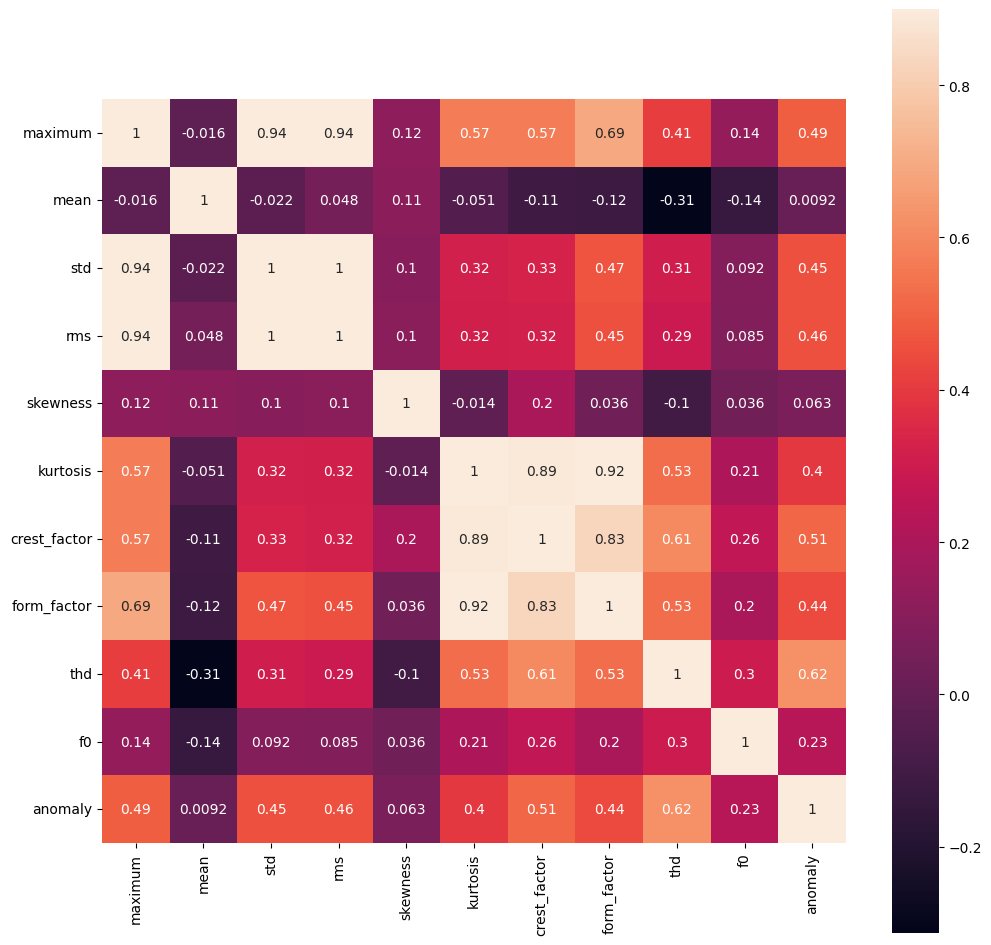
\includegraphics[width=0.8\textwidth]{media/dataset/corr-mat.png}
    \label{fig:figCorrMat}
\end{figure}


\cite{Alvarez2023} definió una matriz de correlación como una tabla que muestra el grado 
de relación lineal entre un conjunto de variables. En forma de matriz cada fila y 
columna representa una variable, está a su vez facilita la visualización conjunta de 
múltiples variables, lo que facilita observar de forma más entendible la exploración de 
los datos de forma gráfica.


En esta matriz se evidencia que los valores en la diagonal principal siempre serán 1 ya 
que se encuentran correlacionadas todas las variables, por otro lado tenemos que los 
valores fuera de la diagonal van de -1 a +1 lo que expresa que mientras más cercano sea 
el valor a +1 más mayor será la relación positiva, es decir, pueden directamente 
proporcionales, por otro lado un valor cercano a -1 indica que no existe una relación 
entre las variables, es decir, pueden ser inversamente proporcionales y un valor cercano 
a 0 indica que no existe una relación clara entre las variables. \cite{Alvarez2023}


Entre muchas de sus ventajas se resaltan la detección de dependencias o redundancia de 
variables, lo cual es muy importante y prioritario en campos como análisis de datos y 
aprendizaje automático y por otro lado nos encontramos que por medio de la implementación
de esta técnica se puede simplificar modelos eliminando variables muy correlacionadas que 
produzcan redundancia en la información. \cite{Alvarez2023}


\begin{figure}[h]
    \caption{Correlación entre la variable objetivo y el resto de parámetros.}
    \centering
    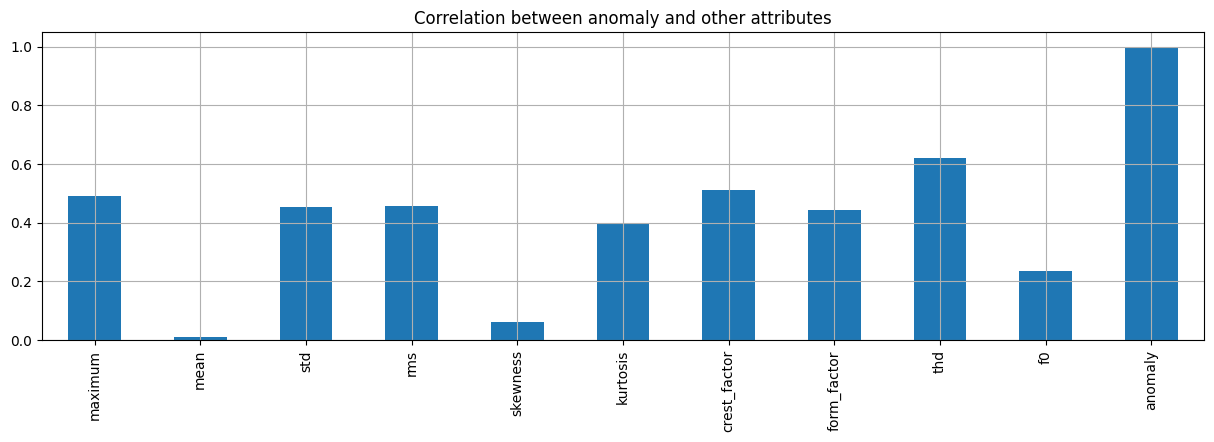
\includegraphics[width=1\textwidth]{media/dataset/corr-mat-target.png}
    \label{fig:figCorrMatTarget}
\end{figure}



Muchas variables tienen relaciones muy fuertes (positivas o negativas) entre sí. 
Por ejemplo,  maximum y minimum tiene una correlación muy cercana a -1. 
Debido a que las señales en el dataset corresponden a vibraciones, se espera que si se 
tiene una vibración con una alta amplitud en uno de los ejes positivos, 
también lo haga en el eje negativo. En el caso de las variables mean a las que se les 
realizó una transformación logarítmica se obtienen correlaciones altas entre 
las variables y su respectiva correlación. 


Finalmente se analiza la relación de correlación entre cada parámetro y la categoría si 
pertenece o no a algún archivo de fallas. La Figura~\ref{fig:figCorrMatTarget} muestra 
la correlación entre cada parámetro y esa variable objetivo. No hay correlaciones fuertes
(mayores a 0.3) entre ninguna variable y anomaly. 
Esto significa que ninguna variable por sí sola explica bien la aparición de anomalías. 
Las variables con mayor asociación, aunque débil, son: \lstinline|log_maximum| (+0.145) y 
\lstinline|log_std| (+0.112), \lstinline|log_minimum| (-0.152) y \lstinline|length| (-0.216).
Variables como \lstinline|mean| y \lstinline|rpm| no aportan relación clara con la anomalía.



\section{Preparación del dataset de entrenamiento}

En esta etapa se estandarizan el conjunto de datos original con fin que los modelos sean 
capaces de utilizar los datos para su entrenamiento y predicción. La salida de esta etapa
son el conjunto de características y etiquetas que utilizarán los modelos de aprendizaje 
supervisado para su entrenamiento y evaluación. Los pasos para la construcción del dataset 
de entrenamiento se visualizan en la Figura~\ref{fig:figGenerationDataset}.


\begin{figure}[h]
    \caption{Etapas para la construcción del dataset de entrenamiento.}
    \centering
    \includegraphics[width=0.9\textwidth]{media/generacion-dataset.drawio.png}
    \label{fig:figGenerationDataset}
\end{figure}


En primer lugar, cada archivo del conjunto de datos contiene mediciones de diferentes 
tipos de acelerómetros. Debido a que los archivos de series de tiempo de condiciones 
normales, no contienen datos del acelerómetros BA. Por esa razón, se ignoran los datos 
provenientes de los acelerómetros de tipo BA, puesto que solo están presente en los 
archivos con datos anómalos. Incluir estos datos genera ruido en el modelo, y en caso 
que se realice una medición en condiciones normales usando el acelerómetro de tipo BA, 
el modelo no sería capaz de clasificarlo correctamente.


Adicionalmente, las series de tiempo de los diferentes archivos no tienen la misma 
longitud, y la cantidad de muestras de los archivos es muy alta. La serie más corta 
tiene más de 60.000 muestras. Con el fin de generar un conjunto de datos con un misma 
longitud y una cantidad mayor de registros, se ha decido tomar segmentos de 2048 
muestras de cada serie.  De esta manera, de un mismo archivo se pueden obtener muchos 
segmentos, que se convertirán en una observación para el entrenamiento o evaluación 
del modelo. 


Los segmentos son seleccionados de forma aleatoria, debido a que hay muchos más archivos 
que tienen datos de condiciones anómalas en comparación a los archivos de datos en 
condiciones normales, de éstos últimos se obtienen más observaciones por archivos que 
de los anteriores. En la salida se obtienen 8192 series de condiciones anómalas de 2048 
muestras cada una y la misma cantidad de series para condiciones normales. 


No es recomendable entrenar directamente un modelo con esos valores crudos de los 
segmentos sin calcular características. En primer lugar, esta alta dimensionalidad de 
los datos hace a los modelos muy grandes, y si la relación entre el número de 
observaciones a entrenar y el número de dimensiones de entrada es muy bajo, son más 
probable que ocurran  efectos negativos como sobreajuste y dificultad para generalizar. 


Por otra parte las series de tiempo suelen tener datos ruidosos y con gran variabilidad 
local. Esto hace que el modelo se ajuste a patrones irrelevantes.  Además, ruido, un 
valor pico o un desplazamiento leve temporal puede tener grandes efectos en los 
resultados del modelo. Extraer features de la serie de tiempo reduce la dimensionalidad, 
mejora la robustez del modelo y facilita la interpretación de resultados. 


Por lo anterior, una vez obtenidos los segmentos, se procede a la generación de las 
características de cada conjunto de muestras. Para esto, se calculan una serie de 
métricas estadísticas descriptivas para cada fila (serie temporal) de la matriz de 
datos. Estas métricas incluyen, el valor máximo de la serie temporal (\texttt{maximum}),
la media de la serie temporal (\texttt{mean}), la desviación estándar de la serie
temporal (\texttt{std}), el valor cuadrático medio de la serie temporal (\texttt{rms}),
la asimetría de la serie temporal (\texttt{skewness}), la relación entre el valor máximo 
y el RMS (\texttt{crest\_factor}) y la relación entre el RMS (\texttt{form\_factor}).

Además, se calculan dos métricas adicionales basadas en el espectro en frecuencia de la señal:
La distorsión armónica total (\texttt{thd}) y la frecuencia fundamental (\texttt{f0}).
Generar características a partir del espectro de frecuencia complementa la información
temporal proveniente de las características anteriores. 


Finalmente, se agrega información adicional a cada fila del DataFrame, como el RPM, el 
tipo de anomalía, el diámetro de la falla, el valor de muestreo y la etiqueta de 
muestreo, así como el nombre del acelerómetro. El resultado final es un DataFrame de 
Pandas que contiene todas las características extraídas de los segmentos de datos, 
listo para ser utilizado en tareas de aprendizaje automático.



\section{Métricas de evaluación utilizadas}


Para determinar las métricas de rendimiento se divide el conjunto de datos en conjuntos 
de entrenamiento y prueba, y que los datos de prueba se utilizan únicamente para 
comparar los modelos, sin participar en el proceso de entrenamiento. La división 
escogida para este experimento es 80\% para entrenamiento y 20\% para prueba. 


\vspace{5mm}
\begin{lstlisting}
df_full_train, df_test = train_test_split(
    df, test_size=0.2, random_state=RANDOM_SEED)
\end{lstlisting}


Los datos se dividen usando la misma semilla aleatoria para garantizar la 
reproducibilidad del experimento, es decir, que todos los modelos tengan exactamente 
los mismos datos de entrenamiento y prueba que tienen los demás, evitando sesgos 
derivados de particiones distintas. Adicionalmente, los datos de entrenamiento se 
dividen aún más en conjuntos de entrenamiento y validación, y durante el proceso de 
entrenamiento se utiliza la técnica de validación cruzada. 


La matriz de confusión constituye el punto de partida para el cálculo de las principales 
métricas de rendimiento en clasificación. En problemas con clases desbalanceadas, la 
matriz de confusión resulta especialmente útil para identificar sesgos hacia una clase 
mayoritaria y analizar con mayor detalle los errores cometidos. A partir de ella se 
derivan la mayoría de las métricas que se utilizan para la evaluación de modelos. En la 
Figura~\ref{fig:figMatrixConfusion} se observa la matriz de confusión que se generará 
de cada modelo entrenado. 



\begin{figure}[h]
    \caption{Matriz de confusión de los modelos calculada con los datos de prueba.}
    \centering
    \includegraphics[width=0.6\textwidth]{media/matrix-confusión.drawio.png}
    \label{fig:figMatrixConfusion}
\end{figure}


\subsubsection{Exactitud}

También llamado Accuracy, es el porcentaje qué indica, del total de predicciones, 
cuántas de las predicciones realizadas durante el entrenamiento tuvieron una predicción 
acertada. Es una de las principales métricas que se utilizan en aprendizaje automático. 
La Ecuación~\eqref{eq:eq2accuracy} describe cómo se calcula esta métrica a partir de 
los valores de la matriz de confusión. 

\begin{equation}\label{eq:eq2accuracy}
\text{Exactitud(Accuracy)} = \frac{TP + TN}{TP + TN + FP + FN}
\end{equation}

Para poder obtener un valor confiable de esta métrica se requiere un conjunto de datos 
correctamente balanceado.  En un escenario donde la clase positiva, por ejemplo, la 
presencia de una falla, es muy poco frecuente en comparación con la clase negativa, el 
modelo podría lograr una alta precisión simplemente prediciendo la clase negativa todo 
el tiempo, sin aprender realmente a identificar correctamente la clase positiva.

\subsubsection{Precisión}

Con esta métrica se busca el grado de dispersión en las predicciones, con el propósito 
de determinar cuántas veces el modelo acertó realmente cuando se predijo la clase 
positiva. La Ecuación~\eqref{eq:eq2precision} describe cómo se calcula esta métrica a 
partir de los valores de la matriz de confusión. 

\begin{equation}\label{eq:eq2precision}
\text{Precisión(Precision)} = \frac{TP}{TP + FP}
\end{equation}

La precisión es clave en situaciones donde los falsos positivos son muy costosos. En el 
caso de la detección de anomalías, realizar un mantenimiento predictivo, puede requerir 
que se suspenda el funcionamiento de una máquina o incluso de la producción. 


\subsubsection{Sensibilidad}

También llamado recall o True Positive Rate, es una métrica valiosa en conjuntos de 
datos desbalanceados. Esta métrica determina, para el total existente de una determinada 
categoría en el conjunto de entrenamiento, cuántas fueron correctamente predichas. La 
Ecuación~\eqref{eq:eq2recall} describe cómo se calcula esta métrica a partir de los 
valores de la matriz de confusión. 

\begin{equation}\label{eq:eq2recall}
\text{Sensibilidad(Recall)} = \frac{TP}{TP + FN}
\end{equation}

La sensibilidad responde a la pregunta: De todas las observaciones de una misma clase, 
¿cuáles fueron predichas correctamente?. Precisión y sensibilidad pueden confundirse 
fácilmente. Pero para dejarlo claro, el número de referencia en precisión es la 
cantidad de predicciones de una categoría (acertadas y no acertadas), mientras qué en 
la sensibilidad el número de referencia es la cantidad real de una categoría en el 
conjunto de entrenamiento.


\subsubsection{F1}

Esta métrica es la combinación de Precisión y sensibilidad, por medio de una media 
armónica. Esta métrica solo puede ser alta si tanto precisión como sensibilidad son 
altas. Si alguno cae, cae toda la métrica. Lo cual nos da una referencia de qué tan 
bueno es el modelo. La Ecuación~\eqref{eq:eq2F1} describe cómo se calcula esta métrica 
a partir de los valores de la matriz de confusión. 

\begin{equation}\label{eq:eq2F1}
F_1 = 2 \cdot \frac{\text{Precisión} \cdot \text{Recall}}{\text{Precisión} + \text{Recall}}
\end{equation}


El F1 mide el equilibrio entre la capacidad del modelo para detectar correctamente los 
positivos (recall) y la capacidad de evitar falsos positivos (precisión). 
Es especialmente útil cuando existe un desequilibrio de clases, como ocurre en detección 
de anomalías, donde las clases suelen estar desbalanceadas. 


\subsubsection{Área bajo la curva ROC}

Esta métrica determina, para distintos umbrales de decisión, la probabilidad de qué un 
conjunto de datos sea clasificado de manera correcta, respecto a cuantos verdaderos 
positivos y falsos positivos tiene. El AUC mide la capacidad del modelo para separar 
clases, independientemente de un umbral específico. Un AUC mayor a 0.9 significa que el 
modelo tiene gran capacidad para identificar patrones anómalos aunque sean poco frecuentes.

A pesar que el conjunto de datos construído contiene un número igual de observaciones 
positivas (presencia de anomalías) y negativas. No se utiliza la exactitud para 
seleccionar al mejor modelo, se optó por elegir al área bajo la curva RoC, puesto que 
esta métrica evalúa qué tan bien el modelo distingue entre condiciones normales y 
anómalas, sin depender de un umbral en particular. 


\section{Modelos de aprendizaje automático}

Para la selección del mejor clasificador binario, se eligen modelos de clasificación 
con el objetivo de predecir si una serie de características corresponden a una anomalía 
o no dentro del conjunto de características. A cada modelo se le aplica un proceso de 
búsqueda de hiperparámetros, lo que permite ajustar sus configuraciones internas y 
obtener un modelo optimizado para alcanzar las mejores métricas de desempeño posibles. 


\subsubsection{Regresión Logística}

El primer modelo de clasificación que se aplica es la regresión logística. Se parte de  
regresión logística ya que es uno de los métodos clásicos de clasificación y de los  más 
efectivos. Otra ventaja de la regresión logística es su fácil interpretación, y por lo 
tanto, el modelo resultante del entrenamiento, puede ser de gran ayuda a la hora de 
obtener una comprensión de los datos. Estos aspectos, junto con su simplicidad, 
justifican su elección como modelo de clasificación.


\vspace{5mm}
\begin{lstlisting}
logistic_regression_params = {
    'dict_vectorizer__sparse': [False],
    'logistic_regression__penalty': ['l2', 'l1', 'elasticnet', None ],
    'logistic_regression__C': [0.1, 1.0, 10.0],
    'logistic_regression__fit_intercept': [True, False],
    'logistic_regression__solver': ['lbfgs']
}
\end{lstlisting}


Además de elegir este modelo, se aplicó la técnica de búsqueda de hiperparametros para 
encontrar aquellos parámetro que permiten al modelo obtener mejores métricas. Se realizó 
utilizando una técnica de validación cruzada, específicamente GridSearchCV, que permite 
explorar de manera exhaustiva el espacio de hiperparámetros definido.

Una vez encontrada la mejor configuración de hiperparámetros, el modelo de Regresión 
Logística entrenado con esos parámetros se puede utilizar para hacer predicciones sobre 
nuevos datos y evaluar su rendimiento en métricas como precisión, exhaustividad, 
puntaje F1, entre otras.


\subsubsection{Naive Bayes}

Adicionalmente, se escogió el modelo de Naive Bayes debido a su simplicidad en la 
construcción de clasificadores, su buen rendimiento en entrenamiento y predicción y su 
fácil interpretabilidad de este tipo de modelos. Este algoritmo permite entender de 
manera directa cómo cada variable contribuye a la predicción de la clase. Esto brinda 
una visión intuitiva sobre las relaciones que existen entre las características de 
entradas y las clases del problema.


\vspace{5mm}
\begin{lstlisting}
naive_bayes_params = {
    'dict_vectorizer__sparse': [False],
    'naive_bayes__var_smoothing': [1e-9, 1e-8, 1e-7, 1e-6]
}
\end{lstlisting}


Con el fin de obtener un mejor modelo se itera con diferentes valores de suavizado 
(smoothing) aplicado a la varianza de cada característica. Un valor más pequeño 
significa que el suavizado es menor.  El objetivo de optimizar este parámetro es 
encontrar la mejor configuración para el modelo de Naive Bayes Gaussiano.


\subsubsection{Clasificador basado en árbol de decisión}

Otro modelo seleccionado fue el modelo de árboles de decisión debido a su capacidad de 
interpretabilidad y a la posibilidad de extraer la importancia de las características 
(feature importance) utilizadas en la clasificación. Este tipo de modelo no solo permite 
visualizar el proceso de decisión de manera jerárquica y comprensible, sino que también 
brinda información valiosa sobre qué variables tienen mayor peso en la predicción. 
Esto resulta especialmente útil para identificar patrones relevantes en los datos y 
para orientar futuras etapas de análisis o recolección de información.


\vspace{5mm}
\begin{lstlisting}
decision_tree_params = {
    'dict_vectorizer__sparse': [False],
    'decision_tree__criterion': ['gini', 'entropy', 'log_loss'],
    'decision_tree__max_depth': [None, 5, 10, 20],
    'decision_tree__min_samples_split': [2, 5, 10],
    'decision_tree__min_samples_leaf': [1, 2, 5]
}
\end{lstlisting}

Así como a los modelos anteriores, también se aplica optimización de hiperparámetros 
con el fin de  de tener un modelo con mejores métricas. El parámetro criterium define 
la función utilizada para medir la calidad de una división de los diferentes árboles de 
decisión y la pureza de los nodos, \lstinline|decision_tree__max_depth|, controla la 
profundidad máxima del árbol de decisión, \lstinline|decision_tree__min_samples_split|  
controla el número mínimo de muestras requeridas para dividir un nodo interno y 
\lstinline|min_samples_leaf| establece el número mínimo de muestras requeridas en 
cada nodo hoja. 


\subsubsection{Clasificador basado en Bosque Aleatorio}

Se seleccionó el modelo de clasificador basado en bosque aleatorio basándose en los 
buenos resultados obtenidos en estudios previos como el de \cite{canovas2017random} 
y \cite{yu2025tkeo}. En diferentes campos, incluyendo la detección de anomalías, 
los modelos de bosque aleatorio han demostrado un rendimiento competitivo en tareas 
de clasificación y regresión debido a su robustez, versatilidad y facilidad de 
entrenamiento. 


\vspace{5mm}
\begin{lstlisting}
random_forest_params = {
    'dict_vectorizer__sparse': [False],
    'random_forest__n_estimators': [100, 200, 500],   
    'random_forest__criterion': ['gini', 'entropy', 'log_loss'],
    'random_forest__max_depth': [None, 5, 10, 20],
    'random_forest__min_samples_split': [2, 5, 10],
    'random_forest__min_samples_leaf': [1, 2, 5],
    'random_forest__bootstrap': [True, False]
}
\end{lstlisting}

La optimización de hiperparámetros es una etapa crucial en el proceso de construcción 
del modelo. algunos parámetros seleccionados para optimizar fueron: el número de árboles 
de decisión (\lstinline|n_estimators|), la función de criterio para dividir los nodos 
(\lstinline|criterion|), la profundidad máxima de los árboles (\lstinline|max_depth|), 
el número mínimo de muestras para dividir un nodo (\lstinline|min_samples_split|), el 
número mínimo de muestras en un nodo hoja (\lstinline|min_samples_leaf|) y si se debe 
utilizar el bootstrap (\lstinline|bootstrap|). 


\subsubsection{CatBoost}

Adicionalmente, se utilizó el modelo de CatBoost y para mejorar el rendimiento del 
modelo, se llevó a cabo un proceso de optimización de hiperparámetros mediante búsqueda 
en malla, ajustando parámetros clave como el número de iteraciones (\lstinline|iterations|),
la tasa de aprendizaje del modelo (\lstinline|learning_rate|), la profundidad de los 
árboles de decisión (\lstinline|depth|), la regularización del modelo 
(\lstinline|l2_leaf_reg|) y el número de divisiones para las características 
(\lstinline|border_count|). Este procedimiento permite encontrar la mejor combinación de 
que maximizan la capacidad predictiva del modelo.


\vspace{5mm}
\begin{lstlisting}
catboost_params = {
    'dict_vectorizer__sparse': [False],
    'catboost__iterations': [100, 200],
    'catboost__learning_rate': [0.01, 0.1],
    'catboost__depth': [4, 6, 8],
    'catboost__l2_leaf_reg': [1, 3, 5],
    'catboost__border_count': [32, 64],
    'catboost__verbose': [False]
}
\end{lstlisting}


\subsubsection{XGBoost}

De los algoritmos de boosting, se incluye también XGBoost ampliamente reconocido por su 
eficiencia y alto rendimiento en tareas de clasificación y regresión. XGBoost ha sido 
ampliamente adoptado en la comunidad de ciencia de datos por su robustez, versatilidad y 
por haber demostrado resultados sobresalientes en aplicaciones de detección de anomalías 
en el mundo real.


\vspace{5mm}
\begin{lstlisting}
xgb_params = {
    'dict_vectorizer__sparse': [False],
    'xgboost__max_depth': [3, 5, 7],
    'xgboost__learning_rate': [0.01, 0.1],
    'xgboost__n_estimators': [100, 200],
    'xgboost__min_child_weight': [1, 3],
    'xgboost__subsample': [0.8, 1.0],
    'xgboost__colsample_bytree': [0.8, 1.0],
    'xgboost__objective': ['binary:logistic']
}
\end{lstlisting}

Para alcanzar un desempeño óptimo, se le aplica un proceso de optimización de 
hiperparámetros mediante búsqueda en malla, ajustando parámetros clave como la 
profundidad máxima de los árboles de decisión (\lstinline|max_depth|), la tasa de 
aprendizaje del modelo (\lstinline|learning_rate|), el número de estimadores 
(\lstinline|n_estimators|), el peso mínimo por nodo (\lstinline|min_child_weight|), la 
fracción de muestras utilizadas en cada árbol (\lstinline|subsample|) y la proporción de 
características consideradas en cada división (\lstinline|colsample_bytree|). 


\subsubsection{LGBM Classifier}

Otro modelo a utilizar es LightGBM (Light Gradient Boosting Machine), un algoritmo de 
boosting basado en árboles que se caracteriza por su alta eficiencia y velocidad de 
entrenamiento en comparación con otros métodos similares. Una de sus principales ventajas 
es que ofrece un muy buen rendimiento en términos de precisión y consumo de memoria. 


\vspace{5mm}
\begin{lstlisting}
lgbm_params = {
    'dict_vectorizer__sparse': [False],
    'lightgbm__n_estimators': [100, 200],
    'lightgbm__learning_rate': [0.05, 0.1],  
    'lightgbm__max_depth': [3, 5],  
    'lightgbm__num_leaves': [7, 15, 31],  
    'lightgbm__min_child_samples': [5, 10],  
    'lightgbm__subsample': [0.8, 1.0],
    'lightgbm__colsample_bytree': [0.8, 1.0],
    'lightgbm__min_split_gain': [0.0, 0.1],  
    'lightgbm__reg_alpha': [0.0, 0.1],  
    'lightgbm__reg_lambda': [0.0, 0.1],  
    'lightgbm__verbose': [-1]  
}
\end{lstlisting}

Para mejorar el desempeño de este modelo, se lleva a cabo una optimización de 
hiperparámetros, ajustando el número de estimadores (\lstinline|n_estimators|), la tasa 
de aprendizaje (\lstinline|learning_rate|), la profundidad máxima de los árboles 
(\lstinline|max_depth|), el número de hojas (\lstinline|num_leaves|), la cantidad mínima 
de muestras por nodo (\lstinline|min_child_samples|), así como la proporción de datos y 
características empleadas en cada iteración (\lstinline|subsample| y 
\lstinline|colsample_bytree|). También se exploraron factores de regularización como 
\lstinline|reg_alpha|, \lstinline|reg_lambda| y el criterio de división 
(\lstinline|min_split_gain|). 



\subsubsection{Clasificador basado en perceptrón multicapa}

Adicionalmente, se agrega un modelo basado en redes neuronales artificiales: Perceptrón 
multicapa. Una de las principales ventajas de este modelo es su capacidad de modelar 
relaciones no lineales complejas entre las variables, lo que las hace especialmente 
potentes en contextos donde los patrones no pueden ser capturados fácilmente por 
algoritmos lineales o basados en árboles. Además, las redes neuronales son modelos 
altamente flexibles y escalables, capaces de ajustarse a distintos volúmenes y tipos de 
datos. Incluso las redes neuronales podrían ser entrenadas directamente con los datos 
crudos. 


\vspace{5mm}
\begin{lstlisting}
mlp_classifier_params = {
    'dict_vectorizer__sparse': [False],
    'mlp_classifier__hidden_layer_sizes': [(32,), (64,), (128,)],
    'mlp_classifier__activation': ['relu', 'tanh', 'logistic'],
    'mlp_classifier__solver': ['adam', 'lbfgs'],
    'mlp_classifier__learning_rate_init': [0.001, 0.01, 0.1],
    'mlp_classifier__batch_size': ['auto', 200],
    'mlp_classifier__learning_rate': ['constant', 'invscaling', 'adaptive'],
    'mlp_classifier__max_iter': [500, 1000, 1500],
    'mlp_classifier__early_stopping': [True, False],
    'mlp_classifier__validation_fraction': [0.2, 0.5]
}
\end{lstlisting}

Al igual que los modelos anteriores, a este modelo se le aplica un proceso de 
optimización de hiperparámetros, evaluando diferentes configuraciones del número de 
neuronas y capas ocultas (\lstinline|hidden_layer_sizes|), funciones de activación 
(\lstinline|activation|), algoritmos de optimización (\lstinline|solver|), tasas de 
aprendizaje iniciales (\lstinline|learning_rate_init|) y estrategias de adaptación del 
aprendizaje (\lstinline|learning_rate|). También se consideraron parámetros relacionados 
con la regularización y la generalización, como el uso de early stopping y la fracción 
de datos destinada a validación (\lstinline|validation_fraction|). 


\subsubsection{Máquinas de soporte vectorial SVM}

Se entrena además un modelo basado en Máquinas de Vectores de Soporte (SVM) para la 
clasificación de anomalías. Este modelo ha sido utilizado en aplicaciones de detección 
de anomalías debido a su capacidad de encontrar hiperplanos óptimos que separan las 
clases con el mayor margen posible. Este algoritmo es especialmente ventajoso en 
escenarios donde las clases no son linealmente separables, ya que puede utilizar 
funciones kernel para proyectar los datos en espacios de mayor dimensión. 


\vspace{5mm}
\begin{lstlisting}
svm_params = {
    'dict_vectorizer__sparse': [False],
    'svm__C': [0.1, 1, 10],                  
    'svm__kernel': ['linear', 'rbf', 'poly'],
    'svm__gamma': ['scale', 'auto'],         
    'svm__degree': [2, 3, 4],                
    'svm__probability': [True]               
}
\end{lstlisting}


Con el fin de optimizar el rendimiento del modelo también se le implementa una búsqueda 
de hiperparámetros. El parámetro \lstinline|C| controla el grado de regularización, 
donde valores más altos reducen los errores de clasificación en entrenamiento pero 
pueden llevar a sobreajuste. El hiperparámetro \lstinline|kernel| define la función de 
transformación que se aplica a los datos, siendo \lstinline|linear|, \lstinline|rbf| y 
\lstinline|poly| algunas de las opciones más comunes. 


Además de los parámetros anteriores, se busca optimizar parámetros como 
\lstinline|gamma| que regula la influencia de cada muestra en el cálculo de la frontera 
de decisión, \lstinline|degree| que especifica el grado del polinomio cuando se 
selecciona el kernel \lstinline|poly|, y el parámetro \lstinline|probability| que 
permite estimar probabilidades de pertenencia a cada clase, lo cual resulta útil en la 
evaluación con métricas basadas en umbrales como el área bajo la curva ROC. 


\subsubsection{KNN}


Finalmente, se entrena un modelo de K-Nearest Neighbors (KNN) con el objetivo de 
evaluar su desempeño en la clasificación de anomalías. 
Este algoritmo se basa en la premisa de que las observaciones similares tienden a 
encontrarse cerca en el espacio de características, lo que lo convierte en una técnica 
intuitiva y de fácil interpretación. Una de sus principales ventajas es que no hace 
suposiciones fuertes sobre la distribución de los datos, además de ser especialmente 
útil en problemas donde la relación entre las variables es compleja y no lineal.


Para mejorar su rendimiento, también se le aplica a este modelo una optimización de 
hiperparámetros. Entre ellos, el hiperparámetro \lstinline|n_neighbors| que define el 
número de vecinos considerados para la clasificación, afectando directamente el sesgo y 
la varianza del modelo. El parámetro \lstinline|weights| define si todos los vecinos 
contribuyen por igual a la decisión (\lstinline|uniform|) o si se les asigna mayor 
importancia a los más cercanos (\lstinline|distance|). Por su parte, \lstinline|metric| 
determina la función de distancia utilizada para calcular la cercanía entre puntos 
(como \lstinline|euclidean|, \lstinline|manhattan| o \lstinline|minkowski|), mientras 
que el hiperparámetro \lstinline|p| ajusta la potencia de la métrica de Minkowski, 
permitiendo simular tanto la distancia Manhattan (\lstinline|p=1|) como la 
Euclídea (\lstinline|p=2|). 


\vspace{5mm}
\begin{lstlisting}
knn_params = {
    'dict_vectorizer__sparse': [False],
    'knn__n_neighbors': [3, 5, 7, 9, 11],     
    'knn__weights': ['uniform', 'distance'],  
    'knn__metric': ['euclidean', 'manhattan', 'minkowski'],  
    'knn__p': [1, 2]  
}
\end{lstlisting}


\section{Desarrollo de la comparativa}


\begin{table}[h]
\caption{Modelos evaluados, parámetros óptimos  y desempeño en validación. Parte I.}
\centering
\renewcommand{\arraystretch}{1.2}
\scriptsize % 🔹 Reduce el tamaño de fuente
\resizebox{\textwidth}{!}{% 🔹 Ajusta la tabla al ancho de la página
\begin{tabular}{|p{3.5cm}|p{9cm}|c|}
    \hline
    \textbf{Modelo} & \textbf{Parámetros óptimos encontrados} & \textbf{RoC-AUC} \\
    \hline
    Regresión logística & 
    \ttfamily
    \begin{minipage}[t]{9cm}
    "dict\_vectorizer\_\_sparse": false,\\
    "logistic\_regression\_\_C": 0.1,\\
    "logistic\_regression\_\_fit\_intercept": false,\\
    "logistic\_regression\_\_penalty": null,\\
    "logistic\_regression\_\_solver": "lbfgs"
    \end{minipage}
    & 0.9980 \\
    \hline
    Naive Bayes &
    \ttfamily
    \begin{minipage}[t]{9cm}
    "dict\_vectorizer\_\_sparse": false,\\
    "naive\_bayes\_\_var\_smoothing": 1e-09
    \end{minipage}
    & 0.9953 \\
    \hline
    Perceptrón Multicapa (MLP) &
    \ttfamily
    \begin{minipage}[t]{9cm}
    "mlp\_classifier\_\_validation\_fraction": 0.2,\\
    "mlp\_classifier\_\_solver": "lbfgs",\\
    "mlp\_classifier\_\_max\_iter": 1500,\\
    "mlp\_classifier\_\_learning\_rate\_init": 0.1,\\
    "mlp\_classifier\_\_learning\_rate": "adaptive",\\
    "mlp\_classifier\_\_hidden\_layer\_sizes": [128],\\
    "mlp\_classifier\_\_early\_stopping": false,\\
    "mlp\_classifier\_\_batch\_size": 200,\\
    "mlp\_classifier\_\_activation": "relu",\\
    "dict\_vectorizer\_\_sparse": false
    \end{minipage}
    & 0.9994 \\
    \hline
    SVM &
    \ttfamily
    \begin{minipage}[t]{9cm}
    "dict\_vectorizer\_\_sparse": false,\\
    "svm\_\_C": 10,\\
    "svm\_\_degree": 4,\\
    "svm\_\_gamma": "auto",\\
    "svm\_\_kernel": "poly",\\
    "svm\_\_probability": true
    \end{minipage}
    & 0.9998 \\
    \hline
    K-NN &
    \ttfamily
    \begin{minipage}[t]{9cm}
    "dict\_vectorizer\_\_sparse": false,\\
    "knn\_\_metric": "manhattan",\\
    "knn\_\_n\_neighbors": 11,\\
    "knn\_\_p": 1,\\
    "knn\_\_weights": "distance"
    \end{minipage}
    & 0.9991 \\
    \hline
\end{tabular}
}
\label{tab:modelosjsonp1}
\end{table}


Para poder comparar los modelos, primero se entrenan con el mismo conjunto de datos para 
garantizar que las diferencias entre las métricas obtenidas al evaluar los modelos 
dependan exclusivamente de los modelos. Adicionalmente, se aplica un proceso de búsqueda 
de hiperparámetros con el fin de encontrar la configuración que ofreciera el mejor 
rendimiento. 


\begin{table}[h]
\caption{Modelos evaluados, parámetros óptimos y desempeño en validación. Parte II.}
\centering
\renewcommand{\arraystretch}{1.2}
\scriptsize % 🔹 Reduce el tamaño de fuente
\resizebox{\textwidth}{!}{% 🔹 Ajusta la tabla al ancho de la página
\begin{tabular}{|p{3.5cm}|p{9cm}|c|}
    \hline
    \textbf{Modelo} & \textbf{Parámetros óptimos encontrados} & \textbf{RoC-AUC} \\
    \hline
    CatBoost &
    \ttfamily
    \begin{minipage}[t]{9cm}
    "catboost\_\_border\_count": 32,\\
    "catboost\_\_depth": 6,\\
    "catboost\_\_iterations": 200,\\
    "catboost\_\_l2\_leaf\_reg": 3,\\
    "catboost\_\_learning\_rate": 0.1,\\
    "catboost\_\_verbose": false,\\
    "dict\_vectorizer\_\_sparse": false
    \end{minipage}
    & \textbf{0.9999} \\
    \hline
    XGBoost &
    \ttfamily
    \begin{minipage}[t]{9cm}
    "dict\_vectorizer\_\_sparse": false,\\
    "xgboost\_\_colsample\_bytree": 0.8,\\
    "xgboost\_\_learning\_rate": 0.1,\\
    "xgboost\_\_max\_depth": 3,\\
    "xgboost\_\_min\_child\_weight": 1,\\
    "xgboost\_\_n\_estimators": 200,\\
    "xgboost\_\_objective": "binary:logistic",\\
    "xgboost\_\_subsample": 1.0
    \end{minipage}
    & \textbf{0.9999} \\
    \hline
    LightGBM &
    \ttfamily
    \begin{minipage}[t]{9cm}
    "lightgbm\_\_verbose": -1,\\
    "lightgbm\_\_subsample": 0.8,\\
    "lightgbm\_\_reg\_lambda": 0.1,\\
    "lightgbm\_\_reg\_alpha": 0.0,\\
    "lightgbm\_\_num\_leaves": 15,\\
    "lightgbm\_\_n\_estimators": 200,\\
    "lightgbm\_\_min\_split\_gain": 0.1,\\
    "lightgbm\_\_min\_child\_samples": 5,\\
    "lightgbm\_\_max\_depth": 3,\\
    "lightgbm\_\_learning\_rate": 0.1,\\
    "lightgbm\_\_colsample\_bytree": 0.8,\\
    "dict\_vectorizer\_\_sparse": false
    \end{minipage}
    & \textbf{0.9999} \\
    \hline
\end{tabular}
}
\label{tab:modelosjsonp2}
\end{table}


Como criterio de comparación para encontrar los parámetros óptimos, se utiliza el área 
bajo la curva ROC (AUC-ROC), métrica que mide la capacidad del modelo para distinguir 
entre clases positivas y negativas. Al optimizar los hiperparámetros con base en esta 
métrica, se garantiza que los modelos seleccionados ofrezcan un equilibrio adecuado 
entre sensibilidad y especificidad, logrando así un desempeño más robusto en la 
detección de anomalías.


\begin{table}[h]
\caption{Modelos evaluados, parámetros óptimos y desempeño en validación. Parte III.}
\centering
\renewcommand{\arraystretch}{1.2}
\scriptsize % 🔹 Reduce el tamaño de fuente
\resizebox{\textwidth}{!}{% 🔹 Ajusta la tabla al ancho de la página
\begin{tabular}{|p{3.5cm}|p{9cm}|c|}
    \hline
    \textbf{Modelo} & \textbf{Parámetros óptimos encontrados} & \textbf{RoC-AUC} \\
    \hline
    Árbol de decisión &
    \ttfamily
    \begin{minipage}[t]{9cm}
    "decision\_tree\_\_criterion": "entropy",\\
    "decision\_tree\_\_max\_depth": 5,\\
    "decision\_tree\_\_min\_samples\_leaf": 1,\\
    "decision\_tree\_\_min\_samples\_split": 10,\\
    "dict\_vectorizer\_\_sparse": false
    \end{minipage}
    & 0.9986 \\
    \hline
    Bosque Aleatorio (Random Forest) &
    \ttfamily
    \begin{minipage}[t]{9cm}
    "random\_forest\_\_n\_estimators": 500,\\
    "random\_forest\_\_min\_samples\_split": 5,\\
    "random\_forest\_\_min\_samples\_leaf": 2,\\
    "random\_forest\_\_max\_depth": 20,\\
    "random\_forest\_\_criterion": "log\_loss",\\
    "random\_forest\_\_bootstrap": false,\\
    "dict\_vectorizer\_\_sparse": false
    \end{minipage}
    & \textbf{0.9999} \\
    \hline
\end{tabular}
}
\label{tab:modelosjsonp3}
\end{table}


Para la mayoría de los modelos se emplea el método Grid Search, que explora de manera 
exhaustiva todas las combinaciones posibles de hiperparámetros definidos. Sin embargo, 
en el caso de Random Forest, LightGBM y Perceptrón Multicapa MLP,  se utiliza Random 
Search, ya que estos algoritmos requieren un mayor esfuerzo computacional durante su 
entrenamiento, y tienen, en su definición de hiperparámetros un conjunto de 
combinaciones más amplio. Esta estrategia permite explorar de forma más eficiente el 
espacio de hiperparámetros y reducir los tiempos de cómputo sin sacrificar la calidad 
del modelo.


Cabe destacar que no fue necesario separar explícitamente el conjunto de datos en 
entrenamiento y validación, ya que se aplica la técnica de validación cruzada 
(cross-validation) al ejecutar la búsqueda de los hiperparámetros. La validación 
cruzada permite evaluar los modelos en múltiples particiones de los datos, y 
proporciona una estimación más confiable del rendimiento del modelo y una reducción 
del riesgo de sesgos y sobreajustes asociados a una única división de entrenamiento y 
prueba. Los resultados de la búsqueda de hiperparámetros: parámetros óptimos para cada 
modelo y valor del área bajo la curva RoC, se observan en la 
Tabla~\ref{tab:modelosjsonp1}, la Tabla~\ref{tab:modelosjsonp2} y la 
Tabla~\ref{tab:modelosjsonp3}.  


Una vez obtenidos los modelos optimizados, se procede a evaluarlos utilizando el 
conjunto de datos de prueba, con el propósito de estimar el desempeño de los modelos 
con datos no vistos durante el entrenamiento. Para esta evaluación se calcularon 
distintas métricas que permiten analizar el rendimiento desde diferentes perspectivas. 


\begin{table}[h]
\caption{Métricas de rendimiento para los diferentes modelos de clasificación.}
\centering
\renewcommand{\arraystretch}{1.2}
\footnotesize
\begin{tabularx}{\textwidth}{|l|X|X|X|X|X|}
\hline
\textbf{Modelo} & 
\centering \textbf{Exactitud \\ (Accuracy)} & 
\centering \textbf{Precisión \\ (Precision)} & 
\centering \textbf{Sensibilidad \\ (Recall)} & 
\centering \textbf{F1} & 
\centering \textbf{Área bajo la \\ curva RoC} \tabularnewline
\hline
Regresión Logística & 0.9893 & 0.9919 & 0.9864 & 0.9892 & 0.9893 \\
\hline
Naive Bayes & 0.9512 & 0.9980 & 0.9031 & 0.9482 & 0.9507 \\
\hline
Árbol de Decisión & 0.9924 & 0.9988 & 0.9858 & 0.9922 & 0.9923 \\
\hline
Bosque Aleatorio & 0.9966 & 0.9994 & 0.9938 & 0.9966 & 0.9966 \\
\hline
CatBoost & 0.9985 & 0.9994 & 0.9975 & 0.9985 & 0.9985 \\
\hline
XGBoost & 0.9988 & 0.9994 & 0.9981 & 0.9988 & 0.9988 \\
\hline
LightGBM & 0.9988 & 1.0000 & 0.9975 & 0.9988 & 0.9988 \\
\hline
Perceptrón Multicapa & 0.9954 & 0.9969 & 0.9938 & 0.9954 & 0.9954 \\
\hline
Support Vector Machine & 0.9960 & 0.9988 & 0.9932 & 0.9960 & 0.9960 \\
\hline
K-NN & 0.9951 & 1.0000 & 0.9901 & 0.9950 & 0.9951 \\
\hline
\end{tabularx}
\label{tab:metricas_modelos}
\end{table}


Entre las métricas calculadas se incluyen la exactitud, que mide la proporción total de 
predicciones correctas; la precisión, que refleja la capacidad del modelo para 
identificar correctamente las observaciones positivas evitando falsos positivos; 
la sensibilidad (también llamada recall), que indica la capacidad para detectar la 
mayor cantidad de anomalías reales; y la métrica F1, que combina precisión y 
sensibilidad en un único valor armónico.


Adicionalmente, se calculó el área bajo la curva ROC (AUC-ROC), una métrica 
ampliamente utilizada en clasificación binaria que evalúa la capacidad del modelo para 
diferenciar entre clases positivas y negativas de manera independiente al umbral de 
decisión. Con este conjunto de métricas fue posible obtener una visión integral del 
rendimiento de los modelos y comparar su capacidad de generalización en la tarea de 
detección de anomalías. Los resultados de las métricas se observan en  
la Tabla~\ref{tab:metricas_modelos}. 



\begin{table}[H]
\caption{Matrices de confusión para los diferentes modelos de clasificación.}
\centering
\renewcommand{\arraystretch}{1.2}
\footnotesize
\begin{tabularx}{\textwidth}{|l|X|X|X|X|X|}
    \hline
    \textbf{Modelo} & 
    \textbf{Vedaderos Positivos (TP)} & 
    \textbf{Falsos Negativos (FN)} & 
    \textbf{Falsos Positvos (FP)} & 
    \textbf{Verdaderos Negativos (TN)} \\
    \hline
    Regresión Logística & 1643 & 22 & 13 & 1599 \\
    \hline
    Naive Bayes & 1653 & 157 & 3 & 1464 \\
    \hline
    Árbol de decisión & 1653 & 23 & 2 & 1598 \\
    \hline
    Bosque Aleatorio & 1655 & 1 & 10 & 1611 \\
    \hline
    CatBoost & 1655 & 1 & 4 & 1617 \\
    \hline
    XGBoost & 1655 & 1 & 3 & 1618 \\
    \hline
     LightGBM & 1656 & 4 & 0 & 1617 \\
    \hline
    Perceptrón Multicapa. & 1651 & 10 & 5 & 1611 \\
    \hline
    Máquina de Soporte Vectorial-SVM & 1654 & 11 & 2 & 1610 \\
    \hline
    kNN & 1656 & 16 & 0 & 1605 \\
    \hline
\end{tabularx}
\label{tab:matrixconff}
\end{table}


Una vez obtenidos los modelos optimizados, se procede a evaluarlos utilizando el 
conjunto de datos de prueba, con el propósito de estimar el desempeño de los modelos 
con datos no vistos durante el entrenamiento. Para esta evaluación se calcularon 
distintas métricas que permiten analizar el rendimiento desde diferentes perspectivas. 


Entre las métricas calculadas se incluyen la exactitud, que mide la proporción total 
de predicciones correctas; la precisión, que refleja la capacidad del modelo para 
identificar correctamente las observaciones positivas evitando falsos positivos; la 
sensibilidad (también llamada recall), que indica la capacidad para detectar la mayor 
cantidad de anomalías reales; y la métrica F1, que combina precisión y sensibilidad en 
un único valor armónico.


Adicionalmente, se calculó el área bajo la curva ROC (AUC-ROC), una métrica ampliamente 
utilizada en clasificación binaria que evalúa la capacidad del modelo para diferenciar 
entre clases positivas y negativas de manera independiente al umbral de decisión. 
Con este conjunto de métricas fue posible obtener una visión integral del rendimiento 
de los modelos y comparar su capacidad de generalización en la tarea de detección de 
anomalías. Los resultados de las métricas se observan en  la Tabla~\ref{tab:matrixconff}. 


\subsection{Interpretación de los modelos}


Además de modelar los datos, los modelos de aprendizaje automático altamente 
interpretables permiten comprender mejor los datos y los fenómenos que representan. 
Los modelos se comportan como codificadores de conocimiento, capaces de resumir la 
información y los patrones ocultos en los datos. A través del proceso de entrenamiento, 
el modelo aprende a identificar relaciones complejas entre las características de entrada 
y a condensar esa información en una estructura matemática que permite predecir si se 
presenta o no una anomalía. 


Algoritmos como la regresión logística, los árboles de decisión y los algoritmos basados 
en Naive Bayes permiten visualizar y cuantificar de forma explícita la relación que 
existe entre las variables de entrada y las predicciones realizadas. Los pesos y 
parámetros que los modelos aprenden a partir del proceso de entrenamiento actúan como 
un mecanismo de síntesis de información del conjunto de datos de entrenamiento. 

\subsubsection{Modelo regresión logística.}

Además de los resultados obtenidos por las métricas de rendimiento, la regresión 
logística ofrece información fácilmente interpretable a través de sus coeficientes. 
Gracias a las características seleccionadas están muy bien representadas por el modelo 
(con métricas cercanas al 99\%) y que éste es capaz de generalizar adecuadamente, 
se puede utilizar los pesos del modelo para hacer un análisis de variables relevantes 
e interpretación del modelo.  


En el modelo de regresión logística, cada coeficiente representa la influencia de una 
característica sobre la probabilidad de que una observación sea clasificada como anomalía, 
la clase positiva. Aquellos coeficientes con un alto valor positivo incrementan la 
probabilidad de que la predicción corresponda a una anomalía, por el contrario una 
probabilidad muy negativa reduce dicha probabilidad. Los coeficientes del modelo de 
regresión logística se pueden observar en la Tabla 5. 


\vspace{5mm}
\begin{lstlisting}[language={}, basicstyle=\ttfamily\footnotesize\color{black}, frame=lines]
accelerometer=DE: -1.8615003172856712
accelerometer=FE: -4.947346656830767
crest_factor: -9.72659641223027
f0: 0.014019224721163898
form_factor: -15.854673788381616
kurtosis: 1.9119920903388743
maximum: 139.43354893582483
mean: 9.803196561082943
rms: 44.7121415768922
skewness: -8.642533319026972
std: 37.831297461008404
thd: 2.7267589007265456
\end{lstlisting}


Gracias a los coeficientes del modelo, se puede inferir que variables como maximum, rms 
y std incrementan la probabilidad de anomalía, mientras que \lstinline|form_factor|, 
skewness y \lstinline|crest_factor| la disminuyen. 
Estas son las variables que más le aportan al modelo y las que más se tienen en cuenta 
a la hora de definir si una observación es o no una anomalía. Si bien el resto de 
características incluidas en el modelo también tienen cierto impacto, su contribución 
relativa es menor, lo que sugiere que su relevancia en el proceso de predicción es 
secundaria


Los resultados anteriores permiten identificar qué variables físicas de este sistema son 
las más relevantes. De acuerdo con este modelo, una mayor amplitud en las vibraciones, 
reflejada en altos valores de maximum y rms, así como una mayor dispersión en los datos 
capturados, evidenciada en el std, constituyen los principales indicios de la presencia 
de anomalías. En términos prácticos, esto significa que cuando se experimenta con picos 
pronunciados o incrementos en la intensidad de las vibraciones, es más probable que esté 
presentando un comportamiento anómalo.


Por otro lado, variables como el \lstinline|form_factor|, el skewness y el 
\lstinline|crest_factor| actúan como factores de corrección, reduciendo la probabilidad 
de anomalía cuando presentan valores elevados, lo cual sugiere que ciertas formas de 
distribución y regularidad en las señales vibracionales son propias de un funcionamiento 
normal. 



\subsubsection{Modelo árbol de decisión.}

Los modelos basados en árboles de decisión son también fácilmente interpretables. 
El árbol de decisión entrenado muestra cómo ciertas características de los datos de 
entrada permiten distinguir entre condiciones normales y anomalías en el sistema. 
Las altas métricas obtenidas con este modelo confirman que las características extraídas 
de la señal capturan de manera efectiva los patrones distintivos entre el funcionamiento 
en condiciones normales y las anomalías del sistema.


Según el árbol de decisión resultante de la etapa de entrenamiento que se observa 
acontinuación, una de las variables con mayor peso en la clasificación es la desviación 
estándar (std), que aparece en los primeros niveles del árbol y actúa como un criterio 
principal de partición. Esta variable también aparece como criterio de partición en 
niveles inferiores. Esto refleja que la dispersión o variabilidad de la señal es un 
indicador clave para identificar anomalías, ya que valores altos de desviación suelen 
estar asociados a comportamientos irregulares o inestables en la dinámica del sistema.

\vspace{5mm}
\begin{lstlisting}[language={}, basicstyle=\ttfamily\footnotesize\color{black}, frame=lines]
|--- std <= 0.08
|   |--- f0 <= 418.50
|   |   |--- mean <= 0.01
|   |   |   |--- class: 1
|   |   |--- mean >  0.01
|   |   |   |--- std <= 0.08
|   |   |   |   |--- truncated branch of depth 2
|   |   |   |--- std >  0.08
|   |   |   |   |--- truncated branch of depth 2
|   |--- f0 >  418.50
|   |   |--- class: 1
|--- std >  0.08
|   |--- std <= 0.09
|   |   |--- skewness <= 0.05
|   |   |   |--- kurtosis <= -0.26
|   |   |   |   |--- class: 1
|   |   |   |--- kurtosis >  -0.26
|   |   |   |   |--- class: 1
|   |   |--- skewness >  0.05
|   |   |   |--- thd <= 2.04
|   |   |   |   |--- truncated branch of depth 2
|   |   |   |--- thd >  2.04
|   |   |   |   |--- class: 1
|   |--- std >  0.09
|   |   |--- class: 1
\end{lstlisting}


Otra variable relevante en este árbol de decisión es la frecuencia fundamental (f0), 
que se utiliza para refinar la clasificación dentro de las ramas donde la desviación 
estándar es baja. Esto sugiere que la distribución de energía en el espectro en 
frecuencia de la señal, y en particular la frecuencia dominante de la vibración, es un 
factor determinante a la hora de diferenciar entre señales en condiciones normales y en 
presencia de anomalías. 


Adicionalmente, otras variables como la media (mean), la asimetría (skewness), la 
curtosis (kurtosis) y la distorsión armónica total (THD) también hacen parte en las 
reglas de decisión, lo que confirma que la forma, la distribución de la señal y su 
contenido armónico aportan información valiosa para su clasificación.



\subsubsection{Modelo naive bayes.}

En primer lugar, las probabilidades a priori muestran que las clases están muy 
balanceadas, resultado de un correcto balance del conjunto de datos, las proporciones 
entre la clase positiva y negativas es casi igual. 
El modelo Native Bayes también aporta información valiosa respecto a los patrones 
encontrados en los datos. La información que se obtuvo se muestra a continuación:  


\vspace{5mm}
\begin{lstlisting}[language={}, basicstyle=\ttfamily\footnotesize\color{black}, frame=lines]
Probabilidades a priori:
Clase 0: 0.4987
Clase 1: 0.5013

Probabilidades condicionales:
Clase 0:
  accelerometer=DE: 0.5003
  accelerometer=FE: 0.4997
  crest_factor: 3.2882
  f0: 259.6311
  form_factor: 1.2471
  kurtosis: -0.1266
  maximum: 0.2406
  mean: 0.0222
  rms: 0.0730
  skewness: -0.0105
  std: 0.0690
  thd: 1.9065
Clase 1:
  accelerometer=DE: 0.5194
  accelerometer=FE: 0.4806
  crest_factor: 4.6022
  f0: 346.1928
  form_factor: 1.3807
  kurtosis: 3.1383
  maximum: 1.3550
  mean: 0.0224
  rms: 0.2841
  skewness: 0.0083
  std: 0.2800
  thd: 3.1732
\end{lstlisting}



Se observa además que las variables adquieren valores medios característicos en cada 
clase. Para la clase negativa (normal), la frecuencia fundamental (\lstinline|f0|) se 
centra alrededor de 259.6 Hz, mientras que en la clase positiva (anomalía) aumenta hasta 
aproximadamente 346.2 Hz. 
Algo similar ocurre con variables como el factor de cresta (\lstinline|crest_factor|), 
que pasa de 3.28 en clase negativa a 4.60 en clase 1. Esto indica que los cambios en la 
frecuencia dominante de vibración y la  presencia de picos más pronunciados en la señal 
son características distintivas de las anomalías.


Por otro lado, según los resultados del modelo, variables como maximun, rms y desviación 
stándard (\lstinline|std|) son relevantes para identificar comportamientos anómalos, 
puesto que mientras que en la clase negativa (normal) destacan valores más bajos de 
variables como el maximum (0.24), el rms (0.073) y la desviación estándar (0.069) en la 
clase positiva, estos parámetros no aparecen explícitamente. Además, diferencias otras 
variables como en el \lstinline|form_factor| y en la asimetría (\lstinline|skewness|) y 
kurtosis también aportan información sobre la forma de la distribución de la señal en 
cada caso.


A pesar que la interpretación de los tres modelos, a primera vista, es diferente para 
algunas variables, la interpretación de los tres modelos se complementa de forma muy 
valiosa, porque cada uno aporta información desde una perspectiva distinta sobre el 
mismo problema de detección de anomalías. La regresión logística aporta claridad sobre 
las tendencias lineales entre las variables del modelo, los árboles de decisión destacan 
relaciones no lineales y reglas de decisión, y Naive Bayes proporciona una visión 
probabilística de las distribuciones de las variables. 


La Regresión Logística muestra que valores altos de maximum, RMS y std aumentan la 
probabilidad de anomalía, mientras que variables como form factor, skewness y crest 
factor la disminuyen.  El Árbol de Decisión, revela interacciones entre variables como 
la desviación estándar (\lstinline|std|), la frecuencia fundamental (\lstinline|f0|) y 
la kurtosis a la hora de realizar predicciones de los datos. Esto complementa la 
regresión logística mostrando no solo qué variables son relevantes, sino también cómo 
interactúan entre sí para determinar una anomalía.


Por último, el Naive Bayes ofrece una perspectiva probabilística sencilla, destacando 
cómo cambian los valores promedio de ciertas variables entre clases. 
El modelo muestra que las anomalías (clase 1) se caracterizan principalmente por 
frecuencias fundamentales más altas, factor de cresta mayores y diferencias en la forma 
estadística de la señal, mientras que las condiciones normales se asocian con valores 
más bajos de amplitud, dispersión y energía de la vibración. 



\chapter{Discusión y análisis de resultados}

Los modelos entrenados tienen muy buenas métricas de rendimiento. 
Los resultados obtenidos en la evaluación de los diferentes modelos de aprendizaje 
automático aplicados a la detección de anomalías muestran un desempeño sobresaliente 
en todas las métricas. 
Al revisar los valores de la Tabla~\ref{tab:metricas_modelos}, se observa que variables 
como la exactitud, 
la precisión, la sensibilidad, el F1-score y el área bajo la curva ROC alcanzan 
valores muy altos, superiores en la mayoría de los casos al 0.99. Esto refleja que los 
errores cometidos por los modelos son mínimos, los modelos logran una detección 
confiable de las anomalías y, por tanto, se cumplen los objetivos planteados en 
este proyecto.


El proceso de generar características a partir de los segmentos de serie de tiempo, 
en lugar de utilizar directamente los datos crudos, contribuyó de manera significativa 
a alcanzar estas métricas tan altas. Al aplicar las transformaciones a los datos y 
obtener indicadores estadísticos y espectrales, se logró capturar información relevante 
que permite a los modelos diferenciar con claridad entre estados normales y anómalos, 
mejorando sustancialmente la capacidad predictiva. Entre los parámetros que más 
contribuyeron a la inferencia de la clasificación están la media, la desviación estándar, 
el RMS, la frecuencia fundamental y la distorsión armónica total.


Con respecto al desempeño específico de los modelos, aquellos basados en técnicas de 
gradient boosting, particularmente XGBoost y LightGBM, alcanzaron las métricas más altas, 
mostrando un equilibrio casi perfecto entre precisión y sensibilidad y obtuvieron las 
métricas más altas entre todos los modelos seleccionados. Sin embargo, incluso modelos 
más simples, como la regresión logística, Naive Bayes o KNN, lograron resultados 
sobresalientes, con métricas por encima del 95\%, lo que indica que los datos están muy 
bien representados y que diferentes enfoques de modelado pueden ser útiles en este 
contexto.


Estos resultados demuestran además de ajustarse a los datos, los modelos permiten 
realizar interpretaciones valiosas sobre los factores más influyentes en la detección 
de anomalías. 
Al realizar un análisis detallado de los modelos de regresión logística, árbol de 
decisión y Naive Bayes, se identifican las variables para los modelos a la hora de 
realizar las predicciones. Esas variables fueron la desviación estándar, el valor 
máximo (pico), el RMS, la frecuencia fundamental y la distorsión armónica total THD. 
Esto le da a algunos modelos una doble ventaja: por un lado, una alta capacidad 
predictiva, y por otro, un mayor entendimiento del comportamiento del sistema.


Finalmente, se hace énfasis en la escasa diferencia entre las métricas de los distintos
modelos, resulta difícil declarar un ganador absoluto únicamente con base en su 
rendimiento. 
Para seleccionar el modelo más adecuado para una implementación práctica, deben 
considerarse otros factores además del rendimiento, como la necesidad de ejecutar el 
sistema en tiempo real, la disponibilidad de recursos computacionales y la 
interpretabilidad del modelo. 


En este sentido,  si se busca un modelo con alta interpretabilidad, se aplica el 
principio de parsimonia para seleccionar modelos como Regresión Logística, Naive Bayes,
o Árboles de Decisión, ya que con éstos es  más fácil de explicar el aporte de cada 
variable al  resultado final.  
Si se requiere rapidez y bajo consumo de cómputo, se aplica el mismo principio, y 
nuevamente modelos como regresión logística o los árboles de decisión suelen ser más 
adecuados porque combinan unas muy buenas métricas con un bajo requerimiento de cómputo.
En escenarios donde se requiera una máxima precisión, modelos más complejos como 
XGBoost o LightGBM se perfilan como la mejor opción.



\chapter{Conclusiones y Trabajo Futuro}

En el presente  trabajo se alcanzaron métricas superiores al 90\% en todos los modelos
evaluados, superando el resultado esperado, lo cual refleja la solidez del enfoque 
planteado para la detección de anomalías en entornos industriales. La etapa de 
preprocesamiento de los datos fue un paso clave: la caracterización de las series de 
tiempo, junto con un adecuado balanceo del dataset y la búsqueda de hiperparámetros, 
permitió que los modelos pudieran generalizar mejor y mostraran robustez frente al 
sobreajuste. Estos resultados confirman la efectividad del pipeline desarrollado para 
transformar datos crudos en características discriminativas útiles para los modelos 
de predicción.


Debido al alto rendimiento alcanzado, todos los modelos evaluados podrían aplicarse en 
una solución in-situ. No obstante, los que obtuvieron las mejores métricas fueron 
XGBoost y LightGBM, confirmando su eficacia como algoritmos de referencia en problemas
de clasificación complejos, y un buen referente para la detección de anomalías. Sin 
embargo, si la implementación requiere simplicidad, interpretabilidad y bajo costo 
computacional, los modelos clásicos como la regresión logística, los árboles de decisión
o Naive Bayes resultan altamente recomendables, ya que ofrecen un equilibrio entre 
eficiencia, precisión e interpretabilidad.


Finalmente, gracias al uso de modelos con mayor interpretabilidad, se identificó que 
variables como los valores pico (\lstinline|maximum|), la desviación estándar 
(\lstinline|std|), el valor RMS (\lstinline|rms|),
la frecuencia fundamental (\lstinline|f0|) y 
la distorsión armónica total (\lstinline|tdh|) son las que más 
aportan a la clasificación de una observación como anomalía. Este hallazgo  además de 
validar la calidad del modelo, proporciona información valiosa para la toma de 
decisiones en el ámbito industrial, al permitir inferir cuáles son los factores físicos
más determinantes en el diagnóstico temprano de fallos.


Como línea de trabajo futuro, una posibilidad interesante es la integración de los 
modelos desarrollados en un PLC (Controlador Lógico Programable) u otro dispositivo
de cómputo industrial. Esto permitiría que la detección de anomalías se ejecute de 
manera automática y en tiempo real dentro del propio entorno productivo. La adaptación
de los algoritmos a este tipo de hardware representa un reto, especialmente en lo 
relacionado con la optimización del uso de recursos computacionales, pero a la vez abre
la puerta a aplicaciones industriales de gran impacto.


Otra línea de investigación a considerar es el diseño de un algoritmo de clasificación
que no solo detecte anomalías, sino que también identifique el tipo específico de falla:
un clasificador multiclase.  Este enfoque aportaría un valor agregado, ya que permitiría
pasar de un sistema de simple diagnóstico (anómalo/no anómalo) a un sistema de prognosis
y clasificación de fallas, capaz de diferenciar entre problemas la gravedad del fallo y 
el lugar donde se presenta. Con ello, las soluciones podrían evolucionar hacia un 
mantenimiento predictivo más preciso y especializado.


% En la Ecuación \eqref{eq:eq1secCTF}


% \begin{equation}\label{eq:eq1secCTF}
% M=\begin{pmatrix}
% 	m_{11}&m_{12}\\
% 	m_{21}&m_{22}
% \end{pmatrix}
% \end{equation}

% En la siguiente Tabla \ref{tab:tab1secCTF}

% \begin{table}[h]
% \centering
% \begin{tabular}{|c|c|}
% 	\hline
% 	1 & 2 \\
% 	\hline
% 	22 & 11 \\
% 	\hline
% \end{tabular}
% \caption{Tabla 1}
% \label{tab:tab1secCTF}
% \end{table}

% En la siguiente Figura \ref{fig:fig1secCTF}

% \begin{figure}[h]
% \includegraphics[width= 0.8\textwidth]{logo_unir}
% \caption{Logo Unir}
% \label{fig:fig1secCTF}
% \end{figure}

% \cite{PIMENTEL2016744} \cite{da_S_Bessa_2023}

%\begin{thebibliography}{a}
%\bibitem{etiqueta} \textsc{Autores},
%\textit{nombre referencia.}
%Información addicional
%\end{thebibliography}

\newpage


\bibliographystyle{apacite}
\bibliography{bibliografia}



\end{document}
